\documentclass[a4paper,11pt]{article}
%----------------------------------------------------------------------------------------
% Use Package's
%----------------------------------------------------------------------------------------

\usepackage[utf8]{inputenc}
\usepackage{amssymb}
\usepackage{amsmath}
\usepackage{amsthm}
\usepackage{pifont}
\usepackage{mathrsfs}
\usepackage{thmbox} %Leftbar command
\usepackage{fancyhdr} % Required for custom headers
\usepackage{lastpage} % Required to determine the last page for the footer
\usepackage{extramarks} % Required for headers and footers
\usepackage{graphicx} % Required to insert images
\usepackage{lipsum} % Used for inserting dummy ''Lorem ipsum'' text into the template
\usepackage{siunitx}
\usepackage{eurosym}
\usepackage{booktabs}
\usepackage{multicol}
\usepackage{float}
\usepackage{wrapfig}
\usepackage{mathtools}
\usepackage{asymptote}
\usepackage{enumitem} % Custom enumerate for e.g. Ring properties
\usepackage{tikz} % Function diagrams
\usepackage{geometry} % Changing textwidth
% - Code listing with color settings - 
\usepackage{listings}
\usepackage{color}
%\usepackage{pdfpages}
\usepackage{todonotes}
% ----------------- biblatex ----------------- 
\usepackage[backend=biber,sorting=ynt]{biblatex}  %,style=alphabetic
\addbibresource{ref.bib}
% -------------------------------------------- 
\definecolor{mygreen}{rgb}{0,0.3,0}
\definecolor{mygray}{rgb}{0.5,0.5,0.5}
\definecolor{mymauve}{rgb}{0.58,0,0.82}
\newcommand{\lsinput}[1]{\lstinputlisting[frame=single, language=Matlab]{#1}}

\newcommand{\mon}[1]{\texttt{#1}}

\lstset{ 
  backgroundcolor=\color{white},   % choose the background color; you must add \usepackage{color} or \usepackage{xcolor}; should come as last argument
  basicstyle=\footnotesize,        % the size of the fonts that are used for the code
  breakatwhitespace=false,         % sets if automatic breaks should only happen at whitespace
  breaklines=false,                 % sets automatic line breaking
  captionpos=b,                    % sets the caption-position to bottom
  commentstyle=\color{mygreen},    % comment style
  deletekeywords={...},            % if you want to delete keywords from the given language
  escapeinside={\%*}{*)},          % if you want to add LaTeX within your code
  extendedchars=true,              % lets you use non-ASCII characters; for 8-bits encodings only, does not work with UTF-8
  firstnumber=1,                   % start line enumeration with line 1000
  frame=single,	                   % adds a frame around the code
  keepspaces=true,                 % keeps spaces in text, useful for keeping indentation of code (possibly needs columns=flexible)
  keywordstyle=\color{blue},       % keyword style
  language=Matlab,                 % the language of the code
  morekeywords={*,...},            % if you want to add more keywords to the set
  numbers=left,                    % where to put the line-numbers; possible values are (none, left, right)
  numbersep=5pt,                   % how far the line-numbers are from the code
  numberstyle=\tiny\color{mygray}, % the style that is used for the line-numbers
  rulecolor=\color{black},         % if not set, the frame-color may be changed on line-breaks within not-black text (e.g. comments (green here))
  showspaces=false,                % show spaces everywhere adding particular underscores; it overrides 'showstringspaces'
  showstringspaces=true,          % underline spaces within strings only
  showtabs=false,                  % show tabs within strings adding particular underscores
  stepnumber=1,                    % the step between two line-numbers. If it's 1, each line will be numbered
  stringstyle=\color{mymauve},     % string literal style
  tabsize=4,	                   % sets default tabsize to 2 spaces
  %title=\lstname                   % show the filename of files included with \lstinputlisting; also try caption instead of title
}


\setcounter{MaxMatrixCols}{20}

%----------------------------------------------------------------------------------------
% Page Layout
%----------------------------------------------------------------------------------------
% Margins
\topmargin=-0.4in
\evensidemargin=0in
\oddsidemargin=0in
\textwidth=6.5in
\textheight=9.7in
\headsep=0.25in 

\linespread{1.1} % Line spacing
\setlength{\parskip}{0.5\baselineskip}

% Set up the header and footer (report)
\fancypagestyle{plain}{%first page of chapters
	\fancyhf{}
	\fancyfoot[LO,RE]{\textsc{Jeroen Lammers}}
	\fancyfoot[RO,LE]{\thepage/\pageref{LastPage}}
	\renewcommand{\headrulewidth}{0pt}
	\renewcommand{\footrulewidth}{0.4pt}
}
\pagestyle{fancy} %otherpages
\fancyhf{}% it clears the header and footer, otherwise the elements of the default "plain" page style will appear
\fancyhead[LO,RE]{} 
\fancyhead[CO,CE]{BSc Project}
\fancyhead[RO,LE]{}
\fancyfoot[LO,RE]{}
\fancyfoot[CO,CE]{Jeroen Lammers}
\fancyfoot[RO,LE]{\thepage/\pageref{LastPage}}
\renewcommand\headrulewidth{0.4pt} % Size of the header rule
\renewcommand\footrulewidth{0.4pt} % Size of the footer rule
\setlength{\parindent}{0ex}
%----------------------------------------------------------------------------------------
% New commands
%----------------------------------------------------------------------------------------
\newcommand{\ap}[2]{\underline{\textbf{AP - #1 :}} #2}
\newcommand{\Question}[3]{\large\textbf{#1 (#2) - \normalsize#3} \vspace{15px} }
\newcommand{\Answer}[1]{\begin{tabular}{l p{.9\textwidth} l} \hspace{.05\textwidth}& #1 &\hspace{.05\textwidth} \end{tabular}}

\newcommand{\C}{\mathbb{C}}
\newcommand{\N}{\mathbb{N}}
\newcommand{\R}{\mathbb{R}}

\newcommand{\Def}[2]{\textbf{\large Def: \normalsize#1}\newline \textit{#2}}
\newcommand{\Thr}[2]{\textbf{\large Thr: \normalsize#1}\newline \textit{#2}}
\newcommand{\Lemma}[2]{\textbf{\large Lem: \normalsize#1}\newline \textit{#2}}
\newcommand{\Prop}[2]{\textbf{\large Prop: \normalsize#1}\newline \textit{#2}}
\newcommand{\Cor}[2]{\textbf{\large Cor: \normalsize#1}\newline \textit{#2}}
\newcommand{\claim}[2]{\textbf{\large Claim: \normalsize#1}\newline \Answer{#2}}
\newcommand{\Example}[2]{\textbf{\large Ex: \normalsize#1}\newline \Answer{#2}}
\newcommand{\Proof}[2]{}%\textbf{Proof: #1}\newline \Answer{#2}}
\newcommand{\Note}[2]{\textbf{\large Note: \normalsize#1}\newline #2}
\newcommand{\Remark}[2]{\textbf{\large Remark: \normalsize#1}\newline #2}
\newcommand{\Ex}[3]{\textbf{\large Exercise: \normalsize#1}\newline #2 \newline \newline \Answer{#3}}
%----------------------------------------------------------------------------------------
% Document
%----------------------------------------------------------------------------------------
\begin{document}
% ----------------------------- Abstract ---------------------------- 
%\setcounter{page}{0}
%
\includepdf{frontpage.pdf}
%\newpage

% belangrijkste gedeelte
% geeft weer waar het over gaat en resultaten
%\section{Abstract}
In this thesis we deal with implementing the existing data informativity framework into a Matlab toolbox. The toolbox has support for both noiseless data as well as data with bounded noise. In the case of noiseless data there are implementations for system identification, stabilisability, controllability, stability, state feedback, deadbeat control, LQR control, dynamic measurement feedback and state identification. In the case of data with bounded noise there are implementations for quadratic stabilisation, $\mathcal{H}_2$ control and $\mathcal{H}_\infty$ control.
% ----------------------------- Introduction  -----------------------
\section{Introduction}
When studying systems and control theory we often focus on finding properties of a given mathematical model. However, in the real world the mathematical model of a system is not always available. In most cases we only have the measurements/data as produced by a system. To combat this, we can use tools from the field of data-driven analysis and control. These tools are able to infer system theoretical properties from the data without explicitly knowing the underlying mathematical model of the system. In this paper we will look at the implementation of the tools provided in \cite{waarde2019data} and \cite{waarde2020noisy}.\newpage
% ----------------------------- Discussion --------------------------
\section{Definitions}
% Abstract of the section
In this section we will introduce the notion of informativity. We will also look at the notation that will be used in the paper to indicate data and sets of systems. 

\subsection{Model classes}
We will start by defining model classes. When considering linear systems in state space form we know that they come in different forms. One of the more general forms is the following.

\begin{align}
	\mathbf{x}(t+1) &= A \mathbf{x}(t) + B \mathbf{u}(t) + \mathbf{w}(t)\\
	\mathbf{y}(t+1) &= C \mathbf{x}(t) + D \mathbf{u}(t)
\end{align}


Let us assume we have a system that has no input ($u$), output ($y$) or noise ($w$) variables and has a state space dimension of $3$. Then the system $\Sigma(A,B,C,D)$ can be described using only an $A$ matrix of size $3$. Intuitively this is a a very different type of system compared to a system that has a state space that is only $1$ dimension and does contain an input, output and noise variable. Hence we define a model class in the following way.

\Def{Model class}{
	A system $\Sigma_1$ is said to be the same model class as $\Sigma_2$ if the dimension of the state space, input space and output space are equivalent between both systems.
}

If we apply this to the previous example we can see that the 2 systems are not of the same model class because their state spaces have different dimensions.

\subsection{Informativity}
% Introducing the set of systems data informativity
Let $\Sigma$ be the set of discrete time models of a given model class and let $\mathcal{S}$ be a system from that model class. Then we know that $\mathcal{S}$ is contained in $\Sigma$. Lets say we want to infer a property from our system $\mathcal{S}$. Then if we show that the property holds for all systems in $\Sigma$ then it would also hold for $\mathcal{S}$. However, due to the size of $\Sigma$ this is not very feasible. Thus we need to reduce $\Sigma$ to a more manageable set. To do this we will use the data generated by $\mathcal{S}$. We will call this data $\mathcal{D}$. We will define the set of all systems of the given model class that are able to generate the data $\mathcal{D}$ by $\Sigma_\mathcal{D}$. By construction we know that $\mathcal{S} \in \Sigma_\mathcal{D} \subseteq \Sigma$.

Suppose we want to show if the true system is controllable, we might not be able to uniquely identify the true system using the data, i.e. $\# \Sigma_\mathcal{D} > 1$. However if we are able to show that every system in the set $\Sigma_\mathcal{D}$ is controllable, then we would also know that the true system is controllable. This is the idea behind data informativity. We say the data $\mathcal{D}$ is informative for a property $\mathcal{P}$ if all systems that describe the data $\Sigma_\mathcal{D}$ have the property $\mathcal{P}$. Let $\Sigma_\mathcal{P} \subseteq \Sigma$ be the set of all systems that have the property $\mathcal{P}$. Then we can reformulate the definition of data informativity as follows.

\Def{Informativity \cite[Def 1]{waarde2019data}}{
	We say that the data $\mathcal{D}$ is informative for a property $\mathcal{P}$ if $\Sigma_\mathcal{D} \subseteq \Sigma_\mathcal{P}$.
}

Suppose that the data describes only the true system, i.e. $\Sigma_{\mathcal{D}} = \{ \mathcal{S} \}$ then we know that if a property $\mathcal{P}$ hold for $\mathcal{S}$ then the data is informative for that property. However, in general, just because $\mathcal{S}$ has a property $\mathcal{P}$ does not immediately imply that the data is informative for $\mathcal{P}$ since the data might describe more then one system. Later on in section (\ref{ExampleOfSingleSystemHavingPropertyButNotInformative}) we will see this in an example where the data describes infinity many systems. 

We will also look at control problems. Suppose we want to see if the property '\textit{is stable in full state feedback with a controller $K$}' holds on the data, then we need to know if all systems are stabilisable by state feedback using the controller $K$. For this we will define the set of systems that are stabilised using state feedback for the controller $K$ as follows:
\[ \Sigma_K = \{ (A,B) \, | \, A + B \, K \mbox{ is stable} \} \]
Then we have that the data is informative if $\Sigma_\mathcal{D} \subseteq \Sigma_K$. We will generalise this using the following definition.

\Def{Informativity for control \cite[Def 3]{waarde2019data}}{
	We say that the data $\mathcal{D}$ is informative for a property $\mathcal{P}(\cdot)$ if there exists a controller $\mathcal{K}$ such that $\Sigma_\mathcal{D} \subseteq \Sigma_{\mathcal{P}(\mathcal{K})}$.
}


\subsection{Data}
% Introducing the notation for data
We will use the following example \cite[Ex 2]{waarde2019data} to give a more precise definition of data.

Lets consider systems from the model class of state space dimension $n$ and input space dimension $m$ without noise or output. Then we know that all systems contained in $\Sigma$ are of the form:
\begin{equation}
	\label{isSystem}
	\mathbf{x}(t+1) = A \mathbf{x}(t) + B \mathbf{u}(t)
\end{equation}
Where $\mathbf{x}(t)$ is the $n$-dimensional state vector and $\mathbf{u}(t)$ is the $m$-dimensional input vector evaluated at time $t$. We will pick a system from $\Sigma$ and call it our 'true' system. We will denote this system as $(A_s , B_s)$. 
We will use our true system to generate/measure the input and state data on $q$ time intervals $\{0,1,\dots,T_i\}$ where $i \in \{1,2,\dots,q\}$. We denote the data collected on one of these intervals as follows:
\begin{align*}
	U^{i}_{-} &= \left[ \begin{array}{cccc} u^{i}(0) & u^{i}(1) & \dots & u^{i}(T_i - 1) \end{array} \right] \\
	X^{i}     &= \left[ \begin{array}{cccc} x^{i}(0) & x^{i}(1) & \dots & x^{i}(T_i) \end{array} \right]
\end{align*}
We will now 'split' the state data into a 'past' and 'future' segment, these are defined similar to $U^i_-$.
\begin{align*}
	X^{i}_{-} &= \left[ \begin{array}{ccc} x^{i}(0) & \dots & x^{i}(T_i - 1) \end{array} \right] \\
	X^{i}_{+} &= \left[ \begin{array}{ccc} x^{i}(1) & \dots & x^{i}(T_i) \end{array} \right]
\end{align*}
With this representation of our state and input data we have that $X^{i}_{+} = A_s \, X^{i}_{-} + B_s \, U^{i}_{-}$. This holds for all measured intervals $i$ of the true system. We will now combine the data of all intervals to get a more general form.
\begin{align*}
	U_{-} &= \left[ \begin{array}{ccc} U^{1}_{-} & \dots & U^{q}_{-} \end{array} \right] &
	X     &= \left[ \begin{array}{ccc} X^{1} & \dots & X^{q} \end{array} \right] \\
	X_{+} &= \left[ \begin{array}{ccc} X^{1}_{+} & \dots & X^{q}_{+} \end{array} \right] &
	X_{-} &= \left[ \begin{array}{ccc} X^{1}_{-} & \dots & X^{q}_{-} \end{array} \right]
\end{align*}
We will define our data $\mathcal{D} := (U_-, X)$. In this example we have that $\Sigma_\mathcal{D} = \Sigma_{(U_-,X)} = \Sigma_{i/s}$ and is defined by:
\begin{equation} \label{isSet}
	\Sigma_{i/s} = \Sigma_{(U_-,X)} = \left\{ (A, B) \, | \, X_{+} = \begin{bmatrix} A & B \end{bmatrix} \begin{bmatrix} X_{-} \\ U_{-} \end{bmatrix} \right\}
\end{equation}

By construction we know that at least the true system $(A_s,B_s)$ is contained in this set.

We can extend this concept to also include the output of a system. Assume we have a system of the form:
\begin{subequations}\label{isoSystem}
	\begin{align}
		\mathbf{x}(t+1) &= A \mathbf{x}(t) + B \mathbf{u}(t) \\
		\mathbf{y}(t+1) &= C \mathbf{x}(t) + D \mathbf{u}(t)
	\end{align}
\end{subequations}

Let us define $Y_-$ in the following way:
\begin{align*}
	Y_-^i &= \begin{bmatrix}	y^i(0) & y^i(1)& \dots & y^i(T_i-1); \end{bmatrix}\\
	Y_- &= \begin{bmatrix} Y_-^1 & Y_-^2 & \dots & Y_-^q	\end{bmatrix}
\end{align*}
Then we can define the set of systems that can describe the data as follows:
\begin{equation}
\label{isoSet} 
\Sigma_{i/o/s} = 
\Sigma_{(U_-,X, Y_-)} = \left\{ (A, B, C, D) \, | \, 
\begin{bmatrix} X_{+} \\ Y_{-} \end{bmatrix} = 
\begin{bmatrix} A & B \\ C & D \end{bmatrix} 
\begin{bmatrix} X_{-} \\ U_{-} \end{bmatrix} \right\} 
\end{equation}

Lastly we will consider systems with bounded noise. These systems will be of the form:
\begin{align} \label{isnSystem}
	\mathbf{x}(t+1) &= A_s \mathbf{x}(t) + B_s \mathbf{u}(t) + \mathbf{w}(t)
\end{align}
For these systems we will only use a single measurement interval. Hence we will define our noise data $W_-$ as follows. \todo{Verify if it really is one interval}
\[ W_- = \begin{bmatrix} w(0) & w(1) & \dots & w(T-1)	\end{bmatrix} \]
Note that $W_-$ is unknown, we only have access to our state and input data generated by these systems. Later, in section (\ref{sectionNoise}) we will go into more detail on how we define the bound on the noise and how we can use this for control.









 \newpage
\section{System identification}
% Abstract section
In this section we will see how we can use the data to identify the true system. We will first consider the theory and then we will see how this can be implemented. Lastly we will consider an example that we will solve using the Matlab function based on the previously discussed algorithm.

% What is Systems identification
\Def{Informative for system identification \cite[Def 5]{waarde2019data}}{
	We say that the data is informative for system identification if the data only describes a single system, i.e. $\Sigma_\mathcal{D} = \{(A_s,B_s)\}$.
}

% Mathematics
\subsection{Theory}
Consider systems of the form (\ref{isSystem}) and let $(U_-,X)$ be the data generated by the true system. Assume that we have recorded $T$ data points, i.e. the dimension of $U_-$ is $m \times T$ and the dimension of $X$ is $n \times (T+1)$. Recall that the set of systems described by this data is given by:
\begin{equation}
	\tag{\ref{isSet}} 
	\Sigma_{(U_-,X)} = \left\{ (A, B) \, | \, X_{+} = \begin{bmatrix} A & B \end{bmatrix} \begin{bmatrix} X_{-} \\ U_{-} \end{bmatrix} \right\} 
\end{equation}
where $\begin{bmatrix} X_{-} \\ U_{-} \end{bmatrix}$ is $(n+m) \times T$. Suppose that the $rank \begin{bmatrix} X_{-} \\ U_{-} \end{bmatrix} = n+m$, then there exists a right inverse $\begin{bmatrix} V_1 & V_2 \end{bmatrix}$ such that $\begin{bmatrix} X_{-} \\ U_{-} \end{bmatrix} \begin{bmatrix} V_1 & V_2 \end{bmatrix} = I_{n+m}$. If we multiply the equation from (\ref{isSet}) with this inverse we get the following:
\begin{equation*}
	X_{+} \begin{bmatrix} V_1 & V_2 \end{bmatrix} = \begin{bmatrix} A & B \end{bmatrix} I_{n+m}
\end{equation*}
Thus if the data is full rank we are able to retrieve the $(A,B)$ pair directly. This results in the following proposition.

% Pseudo code / algorithm
\subsection{Algorithm}
\Prop{\cite[Prop 6]{waarde2019data}}{
	The data $(U_-,X)$ is informative for system identification if and only if:
	\begin{equation} \label{SysIdentRankCond}
		rank \begin{bmatrix} X_{-} \\ U_{-} \end{bmatrix} = n+m 
	\end{equation}
	Furthermore, if (\ref{SysIdentRankCond}) holds, then there exists a right inverse $\begin{bmatrix} V_1 & V_2 \end{bmatrix}$ (as defined above), and for any such right inverse $A_s = X_+ V_1$ and $B_s = X_+ V_2$.
}

Suppose we consider a system without any inputs, then the proposition reduces to checking if $X_-$ has full row rank and finding a right inverse $X_-^\dagger$ of $X_-$. Then we retrieve the system as follows $A_s = X_+ X_-^\dagger$.

let us assume we consider an input, state, output system of the form (\ref{isoSystem}). Recall the set of systems described by the data is given by (\ref{isoSet}):
\begin{equation*} \tag{\ref{isoSet}}
\Sigma_{(U_-,X, Y_-)} = \left\{ (A, B, C, D) \, | \, 
\begin{bmatrix} X_{+} \\ Y_{-} \end{bmatrix} = 
\begin{bmatrix} A & B \\ C & D \end{bmatrix} 
\begin{bmatrix} X_{-} \\ U_{-} \end{bmatrix} \right\} 
\end{equation*}
In this case if the proposition holds, we can also retrieve the $C$ and $D$ matrix by computing $C = Y_- V_1$ and $D = Y_- V_2$.

% Example using function
\subsection{Implementation}
\subsubsection*{Syntax}
\mon{[bool, A] = isInformIdentification(X)} \\
\mon{[bool, A, B] = isInformIdentification(X, U)} \\
\mon{[bool, A, B, C, D] = isInformIdentification(X, U, Y)}

\subsubsection*{Description}
\mon{[bool, A] = isInformIdentification(X)}: returns if the state data is informative for system identification, if it is then \mon{A} contains the \mon{A} is the system matrix in state space representation.\\
\mon{[bool, A, B] = isInformIdentification(X, U)}: returns if the state and input data is informative for system identification, if it is then \mon{A} and \mon{B} are the system matrices in state space representation.\\
\mon{[bool, A, B, C, D] = isInformIdentification(X, U, Y)}: returns if the state, input and output data is informative for system identification, if it is then \mon{A}, \mon{B}, \mon{C} and \mon{D} are the system matrices in state space representation.

\subsubsection*{Input arguments}
\textbf{\mon{X}}: State data matrix of dimension $n \times (T+1)$.\\
\textbf{\mon{U}}: Input data matrix of dimension $m \times T$.\\
\textbf{\mon{Y}}: Output data matrix of dimension $p \times T$.

\subsubsection*{Output arguments}
\textbf{\mon{bool}}: (boolean) True if the data is informative for system identification, false otherwise\\
\textbf{\mon{A}}: (matrix) If the data is informative, it contains the systems \mon{A} matrix, empty otherwise.\\
\textbf{\mon{B}}: (matrix) If the data is informative, it contains the systems \mon{B} matrix, empty otherwise.\\
\textbf{\mon{C}}: (matrix) If the data is informative, it contains the systems \mon{C} matrix, empty otherwise.\\
\textbf{\mon{D}}: (matrix) If the data is informative, it contains the systems \mon{D} matrix, empty otherwise.


\subsection{Examples}
Let us consider the following state and input data:
\begin{align*}
	X &= \begin{bmatrix} 0&1&0 \\ 0&0&1 \end{bmatrix} & U = \begin{bmatrix}	1&0	\end{bmatrix}
\end{align*} 
As we can see the data is not sufficient for system identification:
\begin{equation*}
	rank \begin{bmatrix} X_{-} \\ U_{-} \end{bmatrix}  = rank \begin{bmatrix} 0&1 \\ 0&0 \\ 1&0 \end{bmatrix} = 2 \neq 3
\end{equation*}
This is because the data can be generated by systems of the following form:
\[ \Sigma_{i/s} = \left\{ \left( \begin{bmatrix} 0&a_1 \\ 1&a_2 \end{bmatrix}, \begin{bmatrix} 1 \\ 0 \end{bmatrix} \right) \, | \, a_1, a_2 \in \R \right\} \]
However, if we where to consider the same data with 1 additional data point then the data would be informative for system identification:
\begin{align*}
	X_- &= \begin{bmatrix} 0&1&0 \\ 0&0&1 \end{bmatrix} & U &= \begin{bmatrix}	1&0&\alpha	\end{bmatrix} & rank \begin{bmatrix} 0&1&0 \\ 0&0&1 \\ 1&0&\alpha \end{bmatrix} = 3
\end{align*} 
We can also find the same results using the MatLab functions:
\begin{lstlisting}
X = [0 1 0 ; 0 0 1]; U = [1 0];
[bool, A, B] = isInformIdentification(X, U)
\end{lstlisting}
which will return: \mon{[ false, [], [] ]}.




\newpage
\section{Controllability}
% Abstract section
In this section we will see how we can use the data to conclude if a set of systems are controllable of not. We will first consider the mathematics and then we will see how this can be implemented. Lastly we will consider an example that we will solve using the Matlab function based on the previously discussed algorithm.

% What is controllability
\Def{Informative for controllability \cite[Def 7]{waarde2019data}}{
	We say that the data is informative for controllability if all systems that describe the data are controllable. I.e. $\Sigma_{i/o} \subseteq \left\{ (A,B) \, | \, (A,B) \mbox{ is controllable} \right\}$.
}

% Mathematics
We will base our algorithm on theorem 8 and remark 9 from \cite{waarde2019data}. These give necessary and sufficient conditions for the informativity.

\Thr{Informative for controllability}{
	The data $(U_-, X)$ is informative for controllability if and only if $rank(X_+ - \lambda X_- ) = n$ $\forall \lambda \in \mathbb{C}$.
}

This theorem can be reduced to check a finite amount of complex numbers similar to the Hautus test. We have that the above theorem is equivalent to $rank(X+) = n$ and $rank(X_+ - \lambda X_-) = n$ for all $\lambda \neq 0$ with $\lambda^{-1} \in \sigma(X_- X_+^\dagger)$ with $X_+^\dagger$ being the right inverse of $X_+$ and $\sigma(\cdot)$ denotes the set of eigenvalues of the matrix.

% Proof?
\todo{proof?}

% Pseudo code / algorithm
%This will result in the following pseudo code for the algorithm:
%\begin{lstlisting}
%provide X_ and X+
%if X_ has full row rank
%	for each non zero eigenvalue (lambda) of X_ * X+^-i (X+^-i : right inverse of X+) 
%	check if rank(X+ - \lambda X_) = n
%	if it holds for all eigenvalues then
%		The data is informative for controllability
%else 
%	The data is not informative for controllability
%\end{lstlisting}

% Example using function
\subsection{Examples using implementation}
The algorithm above is implemented in the following functions:
\subsubsection*{Syntax}
\mon{[bool] = isInformControllable(X)} 

\subsubsection*{Description}
\mon{[bool] = isInformControllable(X)}: Returns if the state data from an input-state dataset is informative for controllability.

\subsubsection*{Input arguments}
\textbf{\mon{X}}: State data matrix of dimension $n \times T+1$ from an input-state dataset.

\subsubsection*{Output arguments}
\textbf{\mon{bool}}: (boolean) True if the data is informative for controllability, false otherwise

\subsubsection*{Examples}
We will consider the same data as we did in the example of system identification. Recall the provided data was:
\begin{align*}
X &= \begin{bmatrix} 0&1&0 \\ 0&0&1 \end{bmatrix} & U = \begin{bmatrix}	1&0	\end{bmatrix}
\end{align*} 
For the data to be informative for controllability we need that $X_+ - \lambda X_-$ is full row rank for all $\lambda \in \mathbb{C}$.
\begin{align*}
rank(X_+ - \lambda X_-) = rank\left(\begin{bmatrix} 1&0\\0&1\end{bmatrix} - \begin{bmatrix} 0&\lambda\\0&0\end{bmatrix}\right) = 2
\end{align*}
Hence the data is informative for controllability. 

We can also find the same result by using the Matlab function:
\begin{lstlisting}
X = [0 1 0 ; 0 0 1]; U = [1 0];
[bool] = isInformControllable(X)
\end{lstlisting}
Which will return: \mon{[ 1 ]}.

We can verify the result by considering the systems that generate this data. Recall that the data is generated by systems of the form:
\[ \Sigma_{i/s} = \left\{ \left( \begin{bmatrix} 0&a_1 \\ 1&a_2 \end{bmatrix}, \begin{bmatrix} 1 \\ 0 \end{bmatrix} \right) \, | \, a_1, a_2 \in \R \right\} \]
Thus the controllability matrix is given by:
\[ \begin{bmatrix} B& AB \end{bmatrix} = \begin{bmatrix} 1 & 0 \\ 0 & 1 \end{bmatrix} \]
Since the controllability matrix has full rank we can conclude that systems of this form are indeed controllable.
































\newpage
\section{Stabilisability}
% Abstract section
In this section we will see how we can use the data to conclude if a set of systems are stabilisable or not. We will first consider the mathematics and then we will see how this can be implemented. Lastly we will consider an example that we will solve using the Matlab function based on the previously discussed algorithm.

% What is Stabilisability
\Def{Informative for stabilisability \cite[Def 7]{waarde2019data}}{
	We say that the data is informative for stabilisability if all systems that describe the data are stabilisable. I.e. $\Sigma_{i/o} \subseteq \left\{ (A,B) \, | \, (A,B) \mbox{ is stabilisable} \right\}$.
}

% Mathematics
We will base our algorithm on theorem 8 and remark 9 from \cite{waarde2019data}. These give necessary and sufficient conditions for the informativity.

\Thr{Informative for stabilisability}{
	The data $(U_-, X)$ is informative for stabilisability if and only if $rank(X_+ - \lambda X_- ) = n$ $\forall \lambda \in \mathbb{C}$ such that $|\lambda| \geq 1$.
}

This theorem can be reduced to check a finite amount of complex numbers similar to the Hautus test. We have that the above theorem is equivalent to $rank(X_+ - X_-) = n$ and $rank(X_+ - \lambda X_-) = n$ for all $\lambda \neq 1$ with $(\lambda - 1)^{-1} \in \sigma(X_- (X_+ - X_-)^\dagger)$ with $(X_+ - X_-)^\dagger$ being the right inverse of $(X_+ - X_-)$ and $\sigma(\cdot)$ denotes the set of eigenvalues of the matrix.

% Proof?
%\todo{proof?}

% Pseudo code / algorithm


% Example using function
\subsection{Implementation}
\subsubsection*{Syntax}
\mon{[bool] = isInformStabilisable(X)} 
%\mon{[bool] = isInformStabilisable(X, tolerance)}

\subsubsection*{Description}
\mon{[bool] = isInformStabilisable(X)}: Returns if the data is informative for stabilisability.% Uses default tolerance of \mon{1e-14}.
%\mon{[bool] = isInformStabilisable(X, tolerance)}: Returns if the data is informative for stabilisability given a specific tolerance.  

\subsubsection*{Input arguments}
\textbf{\mon{X}}: State data matrix of dimension $n \times T+1$ from an input-state dataset. \
%\textbf{\mon{tolerance}}: Tolerance used for determining when a value is zero up to machine precision. Default value is \mon{1e-14}.

\subsubsection*{Output arguments}
\textbf{\mon{bool}}: (boolean) True if the data is informative for stabilisability, false otherwise.

\subsection{Examples}
In this example we will consider the same data that we used in system identification and controllability, namely:
\begin{align*}
X &= \begin{bmatrix} 0&1&0 \\ 0&0&1 \end{bmatrix} & U = \begin{bmatrix}	1&0	\end{bmatrix}
\end{align*} 
For the data to be informative for stabilisability we need that $X_+ - \lambda X_-$ is full row rank for all $\lambda \in \mathbb{C}$ such that $|\lambda| \geq 1$.
\begin{align*}
rank(X_+ - \lambda X_-) = rank\left(\begin{bmatrix} 1&0\\0&1\end{bmatrix} - \begin{bmatrix} 0&\lambda\\0&0\end{bmatrix}\right) = 2
\end{align*}
Since the rank condition hold for all $\lambda$ it will also hold for all $|\lambda| \geq 1$. Hence the data is informative for stabilisability. This is consistent with the non data driven theory that controllability implies stabilisability. 

We can also find the same result by using the Matlab function:
\begin{lstlisting}
X = [0 1 0 ; 0 0 1]; U = [1 0];
[bool] = isInformStabilisable(X)
\end{lstlisting}
Which will return: \mon{[ 1 ]}.

We can verify the result by considering the systems that generate this data. Recall that the data is generated by systems of the form:
\[ \Sigma_{i/s} = \left\{ \left( \begin{bmatrix} 0&a_1 \\ 1&a_2 \end{bmatrix}, \begin{bmatrix} 1 \\ 0 \end{bmatrix} \right) \, | \, a_1, a_2 \in \R \right\} \]
Recall that a pair $(A,B)$ is stabilisable if and only if $\begin{bmatrix} A - \lambda I & B \end{bmatrix}$ is full row rank for all $\lambda \in \sigma(A)$ such that $Re(\lambda) \geq 0$. 
\[ rank \left( \begin{bmatrix} A - \lambda I & B \end{bmatrix} \right) = rank \left( \begin{bmatrix} -\lambda & a_1 & 1 \\ 1 & a_2 - \lambda & 0 \end{bmatrix} \right) = 2 \]
Thus the systems that describe the data are stabilisable.\newpage
\section{Stability}
% Abstract section
In this section we will consider data informativity for stability of unforced systems. We will first consider the mathematics and then we will see how it can be implemented. Lastly we will consider an example that we will solve using the Matlab function based on the previously discussed algorithm.

% What is Stability
We will consider our data to be obtained from an unforced system i.e. there was no input. Because of this we will define our data and set of systems as follows:
\begin{align*}
\mathcal{D} &= (X) & \Sigma_s = \Sigma_\mathcal{D} = \left\{ A | X_+ = A \, X_- \right\}
\end{align*}
Using these definitions we can define data informativity for stability as follows.

\Def{Informative for stability}{
	We say the data is informative for stability if all systems describing the data are stable.
}


% Mathematics
\subsection{Mathematics}
However, using our definition of informativity for stabilisability we are able to reduce the condition to showing that the data is informative for identification and that the identified system is stable.

\Cor{\cite{Cor 11}{waarde2019data}}{
	The data $X$ is informative for stability if and only if $X_-$ has full row rank and $X_+ X_-^\dagger$ is stable for any right inverse $X_-^\dagger$. This is equivalent to $\Sigma_s = \left\{A_s\right\}$ and $A_s = X_+ X_-^\dagger$ being stable.
}

% Proof?
%Proof '$\Rightarrow$': \\
%Assume that the data is informative for stability. Then we know that all systems describing the data are stable. We defined the set of systems as follows:
%\begin{align*}
%\Sigma_\mathcal{D} &= \left\{ A | X_+ = A \, X_- \mbox{ s.t. $A$ is stable} \right\} & & \\
%\Sigma_\mathcal{D} &= \left\{ A | X_+ \, X_-^\dagger = A \mbox{ s.t. $A$ is stable} \right\} & \iff& X_- \mbox{ is full row rank} 
%\end{align*}
%Hence $A \in \Sigma_\mathcal{D}$

%Proof '$\Leftarrow$': \\

% Pseudo code / algorithm
%\subsection{Algorithm stability}
%Using the corollary above we can construct the following algorithm for finding if the state data generated from an unforced system is informative for stability.
%\begin{lstlisting}
%provide X_- and X_+
%if the data is informative for system identification
%    identify the system matrix A
%    if A is stable
%    	The data is informative for stability
%else
%	The data is not informative for stability
%\end{lstlisting}

% Example using function
\subsection{Implementation}
The algorithm above is implemented in the following functions:
\subsubsection*{Syntax}
\mon{[bool] = isInformStable(X)}

\subsubsection*{Description}
\mon{[bool] = isInformStable(X)}: Returns if the data of a unforced system is informative for stability.

\subsubsection*{Input arguments}
\textbf{\mon{X}}: State data matrix of dimension $n \times T+1$ from an input-less dataset.

\subsubsection*{Output arguments}
\textbf{\mon{bool}}: (boolean) True if the data is informative for stability, false otherwise

\subsection{Examples}
For this example we will consider the following state data generated by a unforced system:
\[ X = \begin{bmatrix}
1 & \frac{1}{2} & \frac{1}{4} \\ 0 & \frac{1}{2} & \frac{1}{2}
\end{bmatrix} \]
For the data to be informative for stability we need that the data is informative for system identification and that the identified system is stable. The data is informative for system identification if and only if there exists an right inverse $X_-^\dagger$ of $X_-$. Then the identified system is given by $A = X_+ X_-^\dagger$.
\[ A = \begin{bmatrix}
\frac{1}{2} & \frac{1}{4} \\ \frac{1}{2} & \frac{1}{2}
\end{bmatrix} \begin{bmatrix}
1 & \frac{1}{2} \\ 0 & \frac{1}{2}
\end{bmatrix}^{-1} = \begin{bmatrix} \frac{1}{2} & 0 \\ \frac{1}{2} & \frac{1}{2} \end{bmatrix} \]
As we can see from the $A$ matrix its eigenvalues are $\sigma(A) = \{\frac{1}{2}, \frac{1}{2}\}$. Thus the system is stable and hence the data is informative for stability.

We can also find the same result by using the Matlab function:
\begin{lstlisting}
X = [1 0.5 0.25; 0 0.5 0.5];
[bool] = isInformStable(X)
\end{lstlisting}
Which will return: \mon{[ 1 ]}.\newpage
\section{State feedback}
% Abstract section
In this section we will see when en how we can construct a state feedback controller directly from the state-input data. We will first consider the mathematics after which we will look at how we can implement this. Lastly we will look at an example and how we can apply the provided functions.

% What is State feedback
We will consider closed loop state feedback. This means that we want to substitute our input with an input that is based on the state of the system, i.e. $u = K x$ where $K \in \mathbb{R}^{m\times n}$. We will consider the system to be in a stable closed loop form if all eigenvalues of $A + B K$ are stable (inside the unit circle). We can extend this notion to data-driven control as follows.

\Def{Informative for state feedback \cite[Def 12]{waarde2019data}}{
	We say that the data $(U_-,X)$ is informative for stabilization by state feedback if there exists a feedback gain $K$ such that all systems described by the data are part of the set of systems that are stabilised using the gain $K$. I.e. $\Sigma_{i/s} \subseteq \Sigma_K$.
}

We will start by noting that if the data is informative for controllability or stabilisability then there is no guarantee that the there also exists a state feedback controller that stabilises all of the systems at once. However, if we find such a controller that we do know that all the systems described by the data are stabilisable. We will see an example of this later on in this section.

% Mathematics
\subsection{Mathematics}
We will start by looking at the following theorem that gives us necessary and sufficient conditions for informativity for stabilisation by state feedback.

\Thr{\cite[Thr 16]{waarde2019data}}{
The data $(U_-,X)$ is informative for stabilisation by state feedback if and only if the matrix $X_-$ has full row rank and there exists a right inverse $X_-^\dagger$ of $X_-$ such that $X_+ X_-^\dagger$ is stable. Moreover, $K$ is such that $\Sigma_{i/s} \subseteq \Sigma_K$ if and only if $K = U_- X_-^\dagger$, where $X_-^\dagger$ is as described above.
}

% Proof?
From this theorem we can see that the problem can be reduced to finding a specific right inverse such that the systems are stable. From this right inverse we are able to construct the corresponding controller for stabilisation by state feedback.

%Before we take a look at the proof of the theorem we will first note a Lemma that will be used in the proof.

%\Lemma{\cite[Lemma 15]{waarde2019data}}{
%Suppose that the data $(U_-,X)$ are informative for stabilisation by state feedback, and let $K$ be a feedback gain such that $\Sigma_{i/s} \subseteq \Sigma_K$. Then $A_0 + B_0 K = 0$ for all $(A_0, B_0) \in \Sigma_{i/o}^0$. Equivalently: 
%\begin{equation}\label{lemma15} im\begin{bmatrix}I\\K \end{bmatrix} \subseteq im\begin{bmatrix}X_-\\U_- \end{bmatrix} \end{equation}
%}

% Pseudo code / algorithm
%Proof '$\Leftarrow$': \\
%Suppose $X_-$ has full row rank and that there exists a right inverse $X_-^\dagger$ such that $X_+ X_-^\dagger$ is stable. Let us define $K$ as $K = U_- X_-^\dagger$. Let us consider the following:
%\begin{equation} \label{proofStateFeedback}
%X_+ X_-^\dagger = \begin{bmatrix}A&B\end{bmatrix} \begin{bmatrix}X_-&U_-\end{bmatrix} X_-^\dagger = A + B K
%\end{equation}
%This statement hold for all systems describing the data, $(A,B) \in \Sigma_{i/s}$. Hence we can conclude that $K$ is a stabilising controller for all closed loop systems $A + B K$ with $(A,B) \in \Sigma_{i/s}$. Thus $\Sigma_{i/s} \subseteq \Sigma_K$. Hence we can conclude that the data is informative for stabilisation by state feedback. 


%Proof '$\Rightarrow$': \\
%Suppose that the data is informative for stabilisation by state feedback. Let $K$ be such that $A+BK$ is stable for all $(A,B) \in \Sigma_{i/s}$. By \cite[Lemma 15]{waarde2019data} we know (\ref{lemma15}). This implies that $X_-$ has full row rank and there exists a right inverse $X_-^\dagger$ such that:
%\[ \begin{bmatrix}I\\K \end{bmatrix} = \begin{bmatrix}X_-\\U_- \end{bmatrix}X_-^\dagger \] 
%By (\ref{proofStateFeedback}), we find that $A + BK = X_+ X_-^\dagger$, which shows that $X_+ X_-^\dagger$ is stable. Note that the stabilising feedback gain is given by $K = U_- X_-^\dagger$ concluding the proof.

However, in its current form it is not straightforward to compute a right inverse such that $X_+ X_-^\dagger$ is stable. Hence we will use a different version of this theorem that has been rewritten in terms of linear matrix inequalities.

\Thr{\cite[Thr 17]{waarde2019data}}{
The data $(U_-,X)$ is informative for stabilisation by state feedback if and only if there exists a matrix $\Theta \in \mathbb{R}^{T\times n}$ satisfying
\begin{align*}
X_- \Theta &= (X_- \Theta)^\top & \begin{bmatrix} X_- \Theta & X_+ \Theta \\ \Theta^\top X_+^\top & X_- \Theta \end{bmatrix} &> 0
\end{align*}
Moreover, $K$ satisfies $\Sigma_{i/s} \subseteq \Sigma_K$ if and only if $K = U_- \Theta(X_-\Theta)^{-1}$ for some matrix $\Theta$ satisfying the above conditions.
}

This version of the theorem can be implemented using linear matrix inequality solvers such as Yalmip of CVX. The function provided in the toolbox are implemented using Yalmip.

% Example using function
\subsection{Implementation}
\subsubsection*{Syntax}
\mon{[bool, K, diagnostics, info] = isInformStateFeedback(X, U)} \\
\mon{[bool, K, diagnostics, info] = isInformStateFeedback(X, U, tolerance)} \\
\mon{[bool, K, diagnostics, info] = isInformStateFeedback(X, U, tolerance, options)}

\subsubsection*{Description}
\mon{[bool, K, diagnostics, info] = isInformStateFeedback(X, U)}: Returns if the data is informative for stabilisation by state feedback. If so, it also returns a corresponding controller K for closed loop feedback control of the form \mon{A+BK}.\\
\mon{[bool, K, diagnostics, info] = isInformStateFeedback(X, U, tolerance)}: Returns if the data is informative for stabilisation by state feedback given a specific tolerance. If so, it also returns a corresponding controller K for closed loop feedback control of the form \mon{A+BK}.\\
\mon{[bool, K, diagnostics, info] = isInformStateFeedback(X, U, tolerance, options)}: Returns if the data is informative for stabilisation by state feedback given a specific tolerance and a spdsettings object. If so, it also returns a corresponding controller K for closed loop feedback control of the form \mon{A+BK}.

\subsubsection*{Input arguments}
\textbf{\mon{X}}: State data matrix of dimension $n \times T+1$ from an input-state dataset..\\
\textbf{\mon{U}}: Input data matrix of dimension $m \times T$ from an input-state dataset..\\
\textbf{\mon{tolerance}}: Tolerance used for determining when a value is zero up to machine precision. Default value is \mon{1e-14}.\\
\textbf{\mon{options}}: sdpsettings used with the Yalmip solver.

\subsubsection*{Output arguments}
\textbf{\mon{bool}}: (boolean) True if the data is informative for stabilisation by state feedback, false otherwise. If false then the \mon{info} variable can be check to find which condition failed. \\
\textbf{\mon{K}}: (matrix) If the data is informative, it contains a stabilising controller \mon{K} for closed loop control \mon{A+BK}, empty otherwise.\\
\textbf{\mon{diagnostics}}: (struct) Diagnostics from the Yalmip \mon{optimize()} function. \\
\textbf{\mon{info}}: (int) Diagnostic variable use to identify which conditions (if any) failed. The verification is done on the solution obtained from Yalmip. For information about the type of error use the \mon{help} command in Matlab

\subsubsection*{Limitation}
Due to computational limitation in the solver or conditioning of this problem it might be the case that a valid \mon{K} is found even though \mon{bool} is false. This is because we are able to find a solution close enough to the real solution that the results are still satisfactory, even though not all conditions are met. 

\subsection{Examples} \label{ExampleOfSingleSystemHavingPropertyButNotInformative}
We will consider 2 examples in which the data is not informative for system identification. In both of the examples the data is informative for controllability. However in only one of the example will the data be informative for stabilisation by state feedback.

\paragraph*{Example 1}
Let us consider the data from the controllability example.
\begin{align*}
X &= \begin{bmatrix} 0&1&0 \\ 0&0&1 \end{bmatrix} & U = \begin{bmatrix}	1&0	\end{bmatrix}
\end{align*} 
From that example we know that the data is informative for controllability and that the general form of systems that can produce this data is given by:
\[ \Sigma_{i/s} = \left\{ \left( \begin{bmatrix} 0&a_1 \\ 1&a_2 \end{bmatrix}, \begin{bmatrix} 1 \\ 0 \end{bmatrix} \right) \, | \, a_1, a_2 \in \R \right\} \]
Using this we can write the general closed loop form.
\[ x(t+1) = \begin{bmatrix}
-k_1 & a_1 - k_2 \\ 1 & a_2
\end{bmatrix} x(t) \]
Where $k_1$ and $k_2$ are fixed and $a_1 , a_2 \in \mathbb{R}$. Using the first theorem we conclude that the data is not informative for stabilisation by state feedback since $X_-$ does not have full row rank. 

We can also find the same result by using the Matlab function:
\begin{lstlisting}
X = [0 1 0; 0 0 1]; U = [1 0];
[bool] = isInformStateFeedback(X, U)
\end{lstlisting}
Which will return: \mon{[ 0 ]}.

\paragraph*{Example 2 \cite[Example 19]{waarde2019data}}
In the next example we will consider the following data.
\begin{align*}
X &= \begin{bmatrix} 1&0.5&-0.25 \\ 0&1&1 \end{bmatrix} & U = \begin{bmatrix}	-1&-1	\end{bmatrix}
\end{align*}
Since $X_-$ in square and non-singular, we are able to use the first theorem to check if $X_+ X_-^{-1}$ is stable.
\[ X_+ X_-^{-1} = \begin{bmatrix} 0.5&-0.5\\1&0.5 \end{bmatrix} \]
Since its eigenvalues are $\frac{1}{2}(1 \pm \sqrt{2}i)$ we can conclude that $X_+ X_-^{-1}$ is stable. Hence the data is informative for stabilisation by state feedback and the corresponding controller is given by:
\[ K = U_- X_-^{-1} = \begin{bmatrix} -1 & -0.5 \end{bmatrix} \]
We will note that the general form for systems that can produce this data is given by:
\[ \Sigma_{i/s} = \left\{ \left( \begin{bmatrix} 1.5+a_1&0.5 \, a_1 \\ 1 + a_2 &0.5 + 0.5 \, a_2 \end{bmatrix}, \begin{bmatrix} 1 + a_1 \\ a_2 \end{bmatrix} \right) \, | \, a_1, a_2 \in \R \right\} \]
Using this we are able to verify that the closed loop system is indeed stable for all values $a_1$ and $a_2$.
\begin{equation*}
	A + BK = \begin{bmatrix} 1.5+a_1&0.5 \, a_1 \\ 1 + a_2 &0.5 + 0.5 \, a_2 \end{bmatrix} + \begin{bmatrix} - 1 - a_1 &  - 0.5 - 0.5 \, a_1 \\ -a_2 & -0.5 \, a_2 \end{bmatrix} = \begin{bmatrix} 0.5&-0.5\\1&0.5 \end{bmatrix}
\end{equation*}
Which, as we saw earlier, is indeed stable.

We can also find the same result by using the Matlab function:
\begin{lstlisting}
X = [1 0.5 0.25; 0 1 1]; U = [-1 -1];
[bool, K] = isInformStateFeedback(X, U)
\end{lstlisting}
Which will return: \mon{[ 0, [-1 -0.5] ]}. See the limitiation section for more details on why \mon{bool} is false.

%let us consider the following data.
%\begin{align*} X &= \begin{bmatrix} -1&-1&-0.5&0.5&2 \\ 0&0.5&1&1.5&2 \end{bmatrix} & U &= \begin{bmatrix} 1&1&1&1 \end{bmatrix}\end{align*} 
%As we can see $X_-$ has full row rank. Now we need to construct a right inverse such that $X_+ X_-^\dagger$ is stable. 
%
%Since $X_-$ is a wide matrix with full row rank we can find an $F$ and $G$ such that $X_- \begin{bmatrix}F&G\end{bmatrix} = \begin{bmatrix} I_2 & 0_{2\times 2}\end{bmatrix}$ and such that $\begin{bmatrix}F&G\end{bmatrix}$ is non singular. Then the right inverse $X_-^\dagger$ can be written as $X_-^\dagger = F + G * H$ where $H \in \mathbb{R}^{2\times 2}$. (More details about this right inverse will be provided in the next section)
%
%Note that $X_+ X_-^\dagger = X_+ F + X_+ G H$ where $X_+$, $F$ and $G$ are known. Now the problem is reduced to a pole placement optimisation problem. Provided that the pair $(X_+ F, X_+ G)$ is controllable we can pick any eigenvalues for the stabilising controller. However, is mainly the case if the data is also informative for identification as well as controllability \todo{add reasoning}. In most other cases we are not able to pick arbitrary poles for the closed loop system. In this example however, we do have that the pair $(X_+ F, X_+ G)$ is controllable for the following $F$ and $G$.
%\begin{align*}
%F &= \begin{bmatrix}
%	-0.4029 & -0.0288 \\ 
%	-0.3885 &  0.1151 \\ 
%	-0.1727 &  0.2734 \\ 
%	 0.2446 &  0.4460 \\ 
%\end{bmatrix} & 
%G &= \begin{bmatrix}
%-0.0274 &  0.7723 \\ 
%-0.5306 & -0.5219 \\ 
% 0.7758 & -0.1960 \\ 
%-0.3403 &  0.3047 \\ 
%\end{bmatrix}
%\end{align*}
%If we use the \mon{place()} command provided by Matlab to place the eigenvalues at $0.4$ and $0.5$ we get the following $H$.
%\[ H = \begin{bmatrix}-0.1017 & 2.5607 \\ 0.2979 & -7.4989\end{bmatrix} \]
%Recall that the controller was given by $K = U_- X_-^\dagger = U_- (F + G * H) = \begin{bmatrix}-0.6&-2.2\end{bmatrix}$. Using the previously discussed method for system identification we can find that the data is informative for system identification and the the system is given by:
%\begin{align*}
%A &= \begin{bmatrix}
%1&1\\0&1
%\end{bmatrix}&
%B &= \begin{bmatrix}
%0\\0.5
%\end{bmatrix}
%\end{align*}
%Using this we can verify that the eigenvalues of the closed loop system are indeed $\{0.4, 0.5\}$.

%Let us consider the following data:
%\begin{align*} X &= \begin{bmatrix} 1&0.5&-0.25 \\ 0&1&1 \end{bmatrix} & U &= \begin{bmatrix} -1&-1 \end{bmatrix}\end{align*} 
%$X_-$ is a square invertible matrix and if we consider $X_+ X_-^{-1} = \begin{bmatrix} 0.5&-0.5\\1&0.5 \end{bmatrix}$ we can see that it is indeed stable since its eigenvalues are $\frac{1}{2}(1 \pm \sqrt{2}i)$. Hence we can conclude that the data is informative for stabilisation by state feedback.

%We can also solve this problem using the linear matrix inequality. If we pick $\Theta = \begin{bmatrix} 1 & -1 \\ 0 & 2 \end{bmatrix}$ then we can see that it it a solution to the equations. 








\newpage
\section{Deadbeat control}
% Abstract section
In this section we will see how we can find a deadbeat controller using only our data. We will first discusse the underlying mathematics after which we will focus on how we can implement this into code. We will also look at a few examples on how to use the provided function.

% What is Deadbeat
\Def{Informative for deadbeat control \cite[Def 20]{waarde2019data}}{
	We say the data $(U_-,X)$ is informative for deadbeat control if there exists a feedback gain $K$ such that $\Sigma_{i/s} \subseteq \Sigma_K^{nil}$. 
}

In other words, the data is informative if we can stabilise all systems described by the data with a given $K$ such that all closed loop systems only have the zero eigenvalue.

% Mathematics
\subsection{Mathematics deadbeat control}
We will begin by considering the following theorem that gives necessary and sufficient conditions for informativity for deadbeat control.

\Thr{\cite[Thr 21]{waarde20}}{
	The data $(U_-,X)$ is informative for deadbeat control if and only if the matrix $X_-$ has full row rank and there exists a right inverse $X_-^\dagger$ of $X_-$ such that $X_+ X_-^\dagger$ is nilpotent. Moreover, if this condition is satisfied then the feedback gain $K := U_- X_-^\dagger$ yields a deadbeat controller.
}

Using this theorem the problem boils down to finding a suitable right inverse such that $X_- X_-^\dagger$ is nilpotent given that $X_-$ has full row rank. We will consider the following 2 cases, first we will look at the case where $X_-$ is a (full rank) square matrix. Second we will look at the case where $X_-$ is a full row rank wide matrix.
 
First lets assume $X_-$ is a square matrix and has full row rank. Then we know that the only right inverse of $X_-$ is its inverse $X_-^{-1}$. Hence the data is informative for deadbeat control if and only if $X_+ X_-^{-1}$ is nilpotent. 

Now lets assume that $X_-$ is a wide matrix and has full row rank. Then there exists an $F \in \R^{T \times n}$ spanning the row space of $X_-$ and an $G \in \R^{T \times (T-n)}$ spanning the null space of $X_-$ such that $\begin{bmatrix}F&G\end{bmatrix}$ is non singular and $X_- \begin{bmatrix}F&G\end{bmatrix} = \begin{bmatrix}I_n&0_{n\times (T-n)}\end{bmatrix}$. Now let $X^\dagger_- = F + G H$ where $H \in \R^{(T-n) \times n}$ if and only if $X_-^\dagger$ is an right inverse of $X_-$.

Proof '$\Rightarrow$': \\
Let $X^\dagger_- = F + G H$ as described above. Then $X_- X^\dagger_- = X_- F + X_- G H = I_n + 0_{n\times (T-n)} * H = I_n$.

Proof '$\Leftarrow$': \\
\todo{add proof}

Thus finding a right inverse such that $X_+ X_-^\dagger$ is nilpotent is equivalent to finding an $H$ such that $X_+ F + X_+ G H$ is nilpotent. Finding this $H$ can be done using pole placement methods for the pair $(X_+ F, X_+ G)$ and placing all eigenvalues at zero.

% Pseudo code / algorithm
\subsection{Algorithm deadbeat control}
Using the mathematics above we can construct an algorithm for checking if the data is informative for deadbeat control and what the corresponding controller is.

\begin{lstlisting}
provide X_, X+ and U
if X_ has full row rank
	if X_ is square
		if X+ * inv(X_) is nilpotent
			The data is informative for deadbeat control
			K = U_ * inv(X_)
	else
		F : spans rowspace of X_ (pseudo inverse of X_ -> pinv(X_)) 
		G : spans the nullspace of X_ (null(X_))
		if (X+ F, X+ G) is controllable
			H = poleplacement(X+ F, X+ G, [0 ... 0])
			The data is informative for deadbeat control
			K = U_ * (F + G H)
The data is not informative for deadbeat control
\end{lstlisting}

However, due to limitation in Matlabs pole placement function we are not able to implement the algorithm into matlab directly. This is because matlab has 2 functions for pole placement, the \mon{place()} function which does not support poles with high multiplicity, which is hence not useable. The other function \mon{acker()} does support pole placement of poles with high multiplicity, but it is limited to a single dimensional input space. Since $X_+ G$ is an $n \times (T-n)$ matrix, we have that our input space is of dimension $T-n$. However, we are able to circumvent this issue by extending the \mon{acker()} function to support higher dinmensional input. To do this we will use the proof of the sufficientcy in theroem 3.29 as well as lemma 3.31 from \cite{bookTrentelman}.

\subsection{Mathematics extending pole placement}

\Lemma{\cite[Lemma 3.31]{bookTrentelman}}{
	If $(A,B)$ is controllable there exist vectors $u_0 , \dots u_{n-1}$ such that the vectors defined by
	\[ x_0 := 0, \, \, \, x_{k+1} := Ax_k + Bu_k \, \, \, (k = 0, \dots , n-1) \]
	are independent.
}

Assume that the pair $(A,B)$ is controllable, we will use \cite[Lemma 3.31]{bookTrentelman} to construct $u_0, \dots , u_{n-1}$ and $x_0,x_1, \dots ,x_n$. We pick $u_n$ to be arbitrary. Then there exists a unique map $F_0$ such that $F_0 x_k = u_k$ for $k = 1,\dots,n$. We can substitute this to get:
\[ x_{k+1} = Ax_k + BF_0 x_k = (A + BF_0 ) x_k \]
for $k \in [1, \dots, n]$. From this we can see that $x_k = (A+BF_0)^{k-1} x_1$. By construction of lemma 3.31 we have that $x_0 = 0$, thus we have $x_1 = A * 0 + B * u_0 = Bu_0$. We will call this $b = Bu_0 = x_1$. By construction $x_1,\dots,x_n$ are independent. Thus we know that the controlability matrix $\begin{bmatrix}b&(A+BF_0)b&\dots&(A+BF_0)^{n-1}b\end{bmatrix} = \begin{bmatrix}x_1&x_2&\dots&x_n\end{bmatrix}$ is full rank. Hence the pair $(A+BF_0,b)$ is controlable. Since the matrix $b$ is a column vector we can use the \mon{acker()} algorithm to compute a suitable controller $f$ such that $A+BF_0 + bf = A + B(F_0 + u_0 f)$ has apropriate eigenvalues. From this we construct the controller $F = F_0 + u_0 f$ that places the eigenvalues in the chosen positions.

\subsection{Algorithm extending pole placement}
We will now rewrite this into pseudo code:
\begin{lstlisting}
Provide A, B and poles
n : dimension of state space
m : dimension of input space
construct linear independent x_1, ... ,x_n from u_0, ..., u_n-1
pick an arbitrary u_n
F0 := [u1 u2 ... un] * inv([x1 x2 ... xn])
b  := B * u0
f  := acker(A + B F0, b, poles)
K  := F0 + u_0 f
\end{lstlisting}

% Example using function
\subsection{Examples using implementation}
The algorithm above is implemented in the following functions:
\subsubsection*{Syntax}
\mon{[bool, K] = isInformDeadbeatControl(X, U)} 

\subsubsection*{Description}
\mon{[bool, K] = isInformDeadbeatControl(X, U)}: Returns if the data is informative for deadbeat control. If so, it also returns a corresponding controller K for closed loop feedback control of the form \mon{A+BK}.

\subsubsection*{Input arguments}
\textbf{\mon{X}}: State data matrix of dimension $n \times T+1$.\\
\textbf{\mon{U}}: Input data matrix of dimension $m \times T$.

\subsubsection*{Output arguments}
\textbf{\mon{bool}}: (boolean) True if the data is informative for deadbeat control, false otherwise\\
\textbf{\mon{K}}: (matrix) If the data is informative, it contains a stabilising controller \mon{K} for closed loop control \mon{A+BK}, empty otherwise.

\subsubsection{Examples}\newpage
\section{Linear quadratic regulation}
% Abstract section
In this section we will see how we can construct a linear quadratic regulator (LQR) based on a given cost function directly from the input-state data. We will first define what LQR control entails for normal control theory after which we will consider its data-driven dual. We will also see how this data-driven version can be applied to retrieve the controller from the data. Lastly we will see how to solve such a problem both by doing it by hand as well as using the provided Matlab functions.

% What is LQR (normal control)
\subsection{Non data-driven LQR}
We will first revisit the topic of non data-driven LQR. To given an intuitive idea, we want to not only find a solution to the stabilisation problem, we also want to find the best solution given some cost function. Let us consider the discrete-time linear systems of the form $x(t+1) = Ax(t) + Bu(t)$. We will denote the state sequence generated by this system based of a given initial condition $x_0$ and input function $u$ as $x_{x_0 , u}(\cdot)$. We will also define a quadratic cost function associated to the system.
\begin{equation*}
J(x_0 , u) = \sum_{t=0}^{\infty} x^\top (t) Q x (t) + u^\top (t) R u (t)
\end{equation*}
Where $Q$ is symmetric positive semi definite and $R$ is symmetric positive definite. Using these notions want to find for every initial condition $x_0$ an input $\bar{u}$ such that the system stabilises and the cost function is minimised as well as finite, In other words, the $\lim\limits_{t \to \infty} x_{x_0 , \bar{u}}(t) = 0$ given that the cost function $J(x_0 , \bar{u}) \leq J(x_0 , u)$ for all inputs $u$ that cause the system to stabilise. Such an input $\bar{u}$ is called optimal for the given initial condition. As we might expect, an optimal solution does not always exist for every initial condition. Hence we say that an LQR problem is solvable for given $(A,B,Q,R)$ if for every initial condition $x_0$ there exists an optimal solution.

Using the following theorem we can find the solution to the LQR problem. Recall from \cite[Def 3.12]{bookTrentelman} that an eigenvalue is called $(Q,A)$-observable if 
$$rank\begin{pmatrix}A - \lambda I \\ Q \end{pmatrix} = n$$
where $n$ is the dimension of the state space.

\Thr{\cite[Thr 23]{waarde2019data}}
{
	let $Q$ be symmetric positive semi definite and $R$ be symmetric positive definite. Then the following statements hold:
	\begin{enumerate}
		\item If $(A,B)$ is stabilisable, there exists a unique largest real symmetric solution $P^+$ to the discrete-time algebraic Riccati equation
		\begin{equation} \label{DARE}
			P = A^\top P A - A^\top P B (R+B^\top PB)^{-1} B^\top P A + Q
		\end{equation}
		in the sense that $P^+ \geq P$ for every real symmetric $P$ satisfying the discrete-time algebraic Riccati equation. The matrix $P^+$ is positive semi definite.
		\item If, in addition to stabilisability of $(A,B)$, every eigenvalue of $A$ on the unit circle is $(Q,A)$-observable then for every $x_0$ a unique optimal input $\bar{u}$ exists. Furthermore, this input sequence is generated by the feedback law $u = Kx$, where $K$ is given by:
		\begin{equation} \label{LQRK}
			K := -(R+B^\top P^+ B)^{-1} B^\top P^+ A
		\end{equation}
		Moreover, the matrix $A + BK$ is stable.
		\item In fact, the linear quadratic regulator problem is solvable for $(A,B,Q,R)$ if and only if $(A,B)$ is stabilisable and every eigenvalue of $A$ on the unit circle is $(Q,A)$-observable.
	\end{enumerate}
}
If a LQR problem is solvable then we call $K$ the optimal feedback gain for $(A,B,Q,R)$.

% What is LQR (Data driven control)
\subsection{Data-driven LQR}
Now that we have familiarised ourselves with the concept of LQR control we will see how to extend it to data-driven control. We will start by defining the set of systems for which a solution is valid given a feedback gain $K$ and cost matrices $Q$ and $R$.
\[ \Sigma_K^{Q,R} := \left\{ (A,B) \, : \, K \mbox{ is the optimal gain for } (A,B,Q,R) \right\} \]
Using this we can define informativity for linear quadratic regulation as follows.

\Def{Informative for linear quadratic regulation \cite[Def 24]{waarde2019data}}{
	Given matrices $Q$ and $R$, we say that the data $(U_-,X)$ is informative for linear quadratic regulation if there exists feedback gain $K$ such that the optimal gain for all systems is $K$, i.e. $\Sigma_{i/s} \subseteq \Sigma_K^{Q,R}$.
}

We will now consider the following theorem that gives us necessary and sufficient conditions for finding the solution of a data-driven LQR problem.

\Thr{\cite[Thr 26]{waarde2019data}}{
	Let $Q$ be symmetric positive semi definite and $R$ be symmetric positive definite. Then the data $(U_-,X)$ is informative for linear quadratic regulation if and only if at least one of the following two conditions hold:
	\begin{enumerate}
		\item The data $(U_-,X)$ is informative for system identification, that is $\Sigma_{i/s} = \left\{(A_s, B_s)\right\}$, and the linear quadratic regulator problem is solvable for $(A_s,B_s,Q,R)$. In this case, the optimal feedback gain $K$ is of the form (\ref{LQRK}) where $P^+$ is of the form (\ref{DARE}).
		\item For all $(A,B) \in \Sigma_{i/s}$ we have $A = A_s$. Moreover, $A_s$ is stable, $QA_s = 0$, and the optimal feedback gain is given by $K = 0$.
	\end{enumerate}
}

As we can see from the theorem if we are able to identify the system then the data-driven LQR problem reduces to a normal LQR problem for which we have already seen how to solve them. However, there is still the case in which all systems have the same $A = A_s$ matrix, $A_s$ matrix is inherently stable and $QA_s = 0$. We will now look at why this is a valid solution to the LQR problem in the first place.

Assume we have a $A_s$ which is stable and a $Q$ such that $QA_s = 0$. From this point we assume $B$ to be an arbitrary input matrix of dimension $n \times m$. Since $x(t) \in im(A)$ for all $t > 0$ we have that $Qx(t) = 0$ for all $t>0$ if we pick our input function to be zero. Note that if we pick our input to be zero then the input cost of the cost function will also be zero. Hence the cost will be equal to $J(x_0 , u) = x_0^\top Q x_0$, which is finite. Since the system is inherently stable we know that the system will stabilise without any input. Lastly we note that the cost associated with the initial condition is present in all cost sequences generated for different inputs, hence the zero input is the minimal solution to the cost function. Hence this case will provide a valid solution to our LQR problem.

However, even though it is a valid solution it is not easily computable in its current form. Hence we will consider the following theorem which rewrites the condition to one of linear matrix inequalities which can be solved by computational means.

\Thr{\cite[Thr 26]{waarde2019data}}{
	Let $Q$ be symmetric positive semi definite and $R$ be symmetric positive definite. Then the data $(U_-,X)$ is informative for linear quadratic regulation if and only if at least one of the following two conditions hold:
	\begin{enumerate}
		\item The data $(U_-,X)$ is informative for system identification, that is $\Sigma_{i/s} = \left\{(A_s, B_s)\right\}$, and the linear quadratic regulator problem is solvable for $(A_s,B_s,Q,R)$. In this case, the optimal feedback gain $K$ is of the form (\ref{LQRK}) where $P^+$ is of the form (\ref{DARE}).
		\item There exists $\Theta \in \mathbb{R}^{T\times n}$ such that $X_-\Theta = (X_-\Theta)^\top$, $U_-\Theta = 0$, $QX_+\Theta=0$ and 
		\[ \begin{bmatrix} X_-\Theta & X_+\Theta \\ \Theta^\top X_+^\top & X_-\Theta \end{bmatrix} > 0 \]
	\end{enumerate}
}

% Extra notes (optional)


% Example using function
\subsection{Examples using implementation}
The algorithm above is implemented in the following functions:
\subsubsection*{Syntax}
\mon{[bool, K, diagnostics] = isInformLQR(X, U, Q, R)} \\
\mon{[bool, K, diagnostics] = isInformLQR(X, U, Q, R, tolerance)} \\
\mon{[bool, K, diagnostics] = isInformLQR(X, U, Q, R, tolerance, options)}

\subsubsection*{Description}
\mon{[bool, K, diagnostics] = isInformLQR(X, U, Q, R)}: Returns if the data is informative for LQR control. If so, it also returns a corresponding controller \mon{K} for the closed loop feedback control of the form \mon{A+BK}.\\
\mon{[bool, K, diagnostics] = isInformLQR(X, U, Q, R, tolerance)}: Returns if the data is informative for LQR control given a specific tolerance. If so, it also returns a corresponding controller \mon{K} for the closed loop feedback control of the form \mon{A+BK}.\\
\mon{[bool, K, diagnostics] = isInformLQR(X, U, Q, R, tolerance, options)}: Returns if the data is informative for LQR control given a specific tolerance and sdpsettings. If so, it also returns a corresponding controller \mon{K} for the closed loop feedback control of the form \mon{A+BK}.

\subsubsection*{Input arguments}
\textbf{\mon{X}}: State data matrix of dimension $n \times T+1$.\\
\textbf{\mon{U}}: Input data matrix of dimension $m \times T$.\\
\textbf{\mon{Q}}: State cost matrix.\\
\textbf{\mon{R}}: Input cost matrix.\\
\textbf{\mon{tolerance}}: Tolerance used for determining when a value is zero up to machine precision. Default value is \mon{1e-14}.\\
\textbf{\mon{options}}: sdpsettings used with the Yalmip solver.

\subsubsection*{Output arguments}
\textbf{\mon{bool}}: (boolean) True if the data is informative for system identification, false otherwise\\
\textbf{\mon{K}}: (matrix) If the data is informative, it contains a stabilising controller \mon{K} for closed loop control \mon{A+BK}, empty otherwise.\\
\textbf{\mon{diagnostics}}: (struct) Diagnostics from the Yalmip \mon{optimize()} function.


\subsubsection{Examples}
\todo{Todo}\newpage
\section{Dynamic measurement feedback}
% Abstract section
In this section we will consider input-state-output systems and how we can use their data to construct a dynamic measurement feedback controller that stabilises the closed loop system. We will start by recalling what a dynamic measurement feedback controller entails. After which we will consider how we can extend this to data-driven control and how we can define the set of systems as well as informativity. We will then consider necessary and sufficient conditions for finding a dynamic measurement feedback controller for input-state-output data. In the next section we will introduce the concept of state estimation which we will use to extend our theory about dynamic measurement feedback to work using only input and output data.

% Introduce Dynamic feedback control for normal control (reference to Trentelman book)
\subsection{Non-data driven dynamic feedback control}
In this section we will consider discrete time systems that are of the following form.
\begin{subequations}\label{outputSys}
	\begin{align} 
		x(t+1) &= A_s x(t) + B_s u(t) \\
		y(t)   &= C_s x(t) + D_s u(t)
	\end{align}
\end{subequations}

Instead of only using state feedback we will also add an observer to the loop. By combining the observer and the state feedback we get a dynamic measurement controller (see \cite[section 3.12]{bookTrentelman}).
%Instead of using a static feedback gain $K$ we will couple the input of the system to a new linear system. We will call this system the dynamic measurement controller and it is given by:
\begin{align*}
	w(t+1) &= Kw(t) + Ly(t) \\
	u(t)   &= Mw(t)
\end{align*}
Using this controller we can write the closed loop system as:
\begin{align*}
	\begin{bmatrix}
		x(t+1) \\ w(t+1)
	\end{bmatrix}
	&=
	\begin{bmatrix}
		A_s  & B_s M \\ LC_s & K + LD_s M
	\end{bmatrix}
	\begin{bmatrix}
		x(t) \\ w(t)
	\end{bmatrix}
\end{align*}
For this controller to be a stabilising controller we need that the closed loop system is stable.

\subsection{Data-driven stabilisation by dynamic measurement feedback}
Recall that the $\Sigma_{i/o/s}$ is given by:
\begin{equation}
\tag{\ref{isoSet}} 
\Sigma_{i/o/s} = \left\{ (A, B, C, D) \, | \, 
\begin{bmatrix} X_{+} \\ Y_{-} \end{bmatrix} = 
\begin{bmatrix} A & B \\ C & D \end{bmatrix} 
\begin{bmatrix} X_{-} \\ U_{-} \end{bmatrix} \right\} 
\end{equation}
We will now define the set of systems to be stabilised using the dynamic feedback controller $(K,L,M)$ as follows.
\[
	\Sigma_{K,L,M} = \left\{ (A,B,C,D) \, | \, \begin{bmatrix} A & BM \\ LC & K + LDM \end{bmatrix} \mbox{ is stable} \right\}
\]
Using these sets we can construct a definition for informativity for dynamic measurement feedback.

\Def{Informative for stabilisation by dynamic measurement feedback \cite[Def 32]{waarde2019data}}{
	We say that the data $(U_-, X, Y_-)$ is informative for stabilisation by dynamic measurement feedback if there exists matrices $K$, $L$ and $M$ such that all systems described by the data are stabilised using the dynamic measurement controller $(K,L,M)$. I.e. $\Sigma_{i/o/s} \subseteq \Sigma_{K,L,M}$.
}

We will start by assuming that our input data is of full rank. The following theorem provides us with a condition on when the data is informative for dynamic measurement feedback.

\Thr{\cite[Thr 34]{waarde2019data}}{
	Consider the data $(U_-,X,Y_-)$ and assume that $U_-$ has full row rank. Then the data is informative for stabilisation by dynamic measurement feedback if and only if the following conditions are satisfied:
	\begin{enumerate}
		\item We have that the data is informative for system identification.
			\[ \Sigma_{i/o/s} = \left\{ (A_s, B_s, C_s, D_s) \right\} \]
		\item The pair $(A_s,B_s)$ is stabilisable and the pair $(C_s,A_s)$ is detectable.
	\end{enumerate}
	Moreover, if the above conditions are satisfied, a stabilising controller $(K,L,M)$ can be constructed as follows:
	\begin{enumerate}
		\item Take $M$ such that $A_s + B_sM$ is stable.
		\item Take $L$ such that $A_s - LC_s$ is stable.
		\item Define $K = A_s + B_sM - LC_s - LD_sM$.
	\end{enumerate}
}

Although the results of this theorem is useful it is quite limited in applicability. Hence we will consider the following lemma that we will use to remove the full input rank restriction from the previous theorem.

\Lemma{\cite[Lem 33]{waarde2019data}}{
	Consider the data $(U_-, X, Y_-)$ and the corresponding set $\Sigma_{i/o/s}$. Let the rank $U_-$ be $k$ where $k \leq m$. Then we can find a matrix $S$ of size $m \times k$ such that $S$ has full column rank and $U_- = S \bar{U}_-$ where $\bar{U}_-$ has full row rank of dimension $k$. 
	Then the data $(U_-,X,Y_-)$ is informative for stabilisation by dynamic measurement feedback if and only if the data $(\bar{U}_-, X, Y_-)$ is informative for stabilisation by dynamic measurement feedback. 
	Moreover, if we define $\bar{\Sigma}_{i/o/s}$ to be the set of systems that are described by the reduced data $(\bar{U}_-,X,Y_-)$ , $(\bar{K},\bar{L},\bar{M})$ is the corresponding dynamic measurement controller and $S^\dagger$ is the left inverse of $S$, then 
	\begin{align*}
		\Sigma_{i/o/s} \subseteq \Sigma_{K,L,M} &\Longrightarrow \bar{\Sigma}_{i/o/s} \subseteq \Sigma_{K,L,S^\dagger M} \\
		\bar{\Sigma}_{i/o/s} \subseteq \Sigma_{\bar{K},\bar{L},\bar{M}} &\Longrightarrow \Sigma_{i/o/s} \subseteq \Sigma_{\bar{K},\bar{L},S\bar{M}}
	\end{align*}
}

Using this duality we are able to extend the precious theorem to work for cases in which the input data is not full rank.

\Cor{\cite[Cor 36]{waarde2019data}}{
	Let $S$ be any full column rank matrix such that $U_- = S \bar{U}_-$ with $\bar{U}_-$ full row rank $k$. The data $(U_-,X,Y_-)$ is informative for stabilisation by dynamic measurement feedback if and only if the following two conditions are satisfied:
	\begin{enumerate}
		\item $(\bar{U}_-,X,Y_-)$ is informative for system identification.
			\[ \Sigma_{i/o/s} = \left\{ (\bar{A}_s, \bar{B}_s, \bar{C}_s, \bar{D}_s) \right\} \]
		\item The pair $(\bar{A}_s,\bar{B}_s)$ is stabilisable and the pair $(\bar{C}_s,\bar{A}_s)$ is detectable.
	\end{enumerate}
	Moreover, if the above conditions are satisfied, a stabilising controller $(K,L,M)$ is constructed as follows:
	\begin{enumerate}
		\item Let $\bar{M}$ be such that $\bar{A}_s + \bar{B}_s \bar{M}$ is stable.
		\item Take $M = S \bar{M}$.
		\item Take $L$ such that $\bar{A}_s - L \bar{C}_s$ is stable.
		\item Define $K = \bar{A}_s + \bar{B}_s \bar{M} - L\bar{C}_s - L\bar{D}_s\bar{M}$.
	\end{enumerate}
}

Note that if we where to substitute $U_- = S\bar{U}_-$ in the state space equations we get the following.
\[ \begin{bmatrix} X_{+} \\ Y_{-} \end{bmatrix} = 
\begin{bmatrix} A_s & B_s \\ C_s & D_s \end{bmatrix} 
\begin{bmatrix} X_{-} \\ U_{-} \end{bmatrix} = 
%\begin{bmatrix} A_s & B_s \\ C_s & D_s \end{bmatrix} 
%\begin{bmatrix} I \\ S \end{bmatrix}
%\begin{bmatrix} X_{-} \\ \bar{U}_{-} \end{bmatrix} = 
\begin{bmatrix} A_s & B_sS \\ C_s & D_sS \end{bmatrix} 
\begin{bmatrix} X_{-} \\ \bar{U}_{-} \end{bmatrix}
 \]
If we assume that the state and reduced input data have full rank then we can see that we are able to identify the systems $A_s$ and $C_s$ matrices uniquely. However we are only able to indentify the systems $B_s$ and $D_s$ matrices up to similarity transformation $S$.

% Example using function
\subsection{Implementation}
The algorithm above is implemented in the following functions:
\subsubsection*{Syntax} 
\mon{[bool, K, L, M] = isInformDynamicMeasurementFeedback(X, U, Y)} \\
\mon{[bool, K, L, M] = isInformDynamicMeasurementFeedback(X, U, Y, polesM, polesL)}

\subsubsection*{Description} 
\mon{[bool, K, L, M] = isInformDynamicMeasurementFeedback(X, U, Y)}: Returns if the data is informative for dynamic measurement feedback. If the data is informative the function also returns a controller \mon{(K,L,M)} where the poles of \mon{M} and \mon{L} are placed at \mon{\{0/n, ..., (n-1)/n\}} where \mon{n} is the dimension of the state space.\\
\mon{[bool, K, L, M] = isInformDynamicMeasurementFeedback(X, U, Y, polesM, polesL)}: Returns if the data is informative for dynamic measurement feedback. If the data is informative the function also returns a controller \mon{(K,L,M)} where the poles of \mon{M} and \mon{L} are placed at the provided locations.

\subsubsection*{Input arguments} 
\textbf{\mon{X}}: State data matrix of dimension $n \times T+1$ from a input/state/output dataset.\\
\textbf{\mon{U}}: Input data matrix of dimension $m \times T$ from a input/state/output dataset.\\
\textbf{\mon{Y}}: Output data matrix of dimension $p \times T$ from a input/state/output dataset.\\
\textbf{\mon{polesM}}: An array containing the desired pole locations for \mon{A + BM}.\\
\textbf{\mon{polesL}}: An array containing the desired pole locations for \mon{A - LC}.

\subsubsection*{Output arguments} 
\textbf{\mon{bool}}: (boolean) True if the data is informative for dynamic measurement feedback, false otherwise\\
\textbf{\mon{K}}: (matrix) The $K$ matrix of the dynamic measurement feedback controller.\\
\textbf{\mon{L}}: (matrix) The $L$ matrix of the dynamic measurement feedback controller.\\
\textbf{\mon{M}}: (matrix) The $M$ matrix of the dynamic measurement feedback controller.

\subsection{Examples}
We will consider an example in which the input data is not full rank. We will consider the following data.
\begin{align*}
	U_- &= \begin{bmatrix} 1&-1&2&0\\-1&1&-2&0 \end{bmatrix} \\
	X &= \begin{bmatrix} 1&3&2&1&-4\\0&3&-5&-6&-2 \end{bmatrix} \\
	Y_- &= \begin{bmatrix} 2&6&4&2 \end{bmatrix} \\
\end{align*}
We will start by finding a matrix $S$ such that $U_- = S \bar{U}_-$ where $S$ has full column rank and $\bar{U}_-$ has full row rank.
\begin{align*}
	U_- &= \begin{bmatrix} 1 \\ -1 \end{bmatrix} \begin{bmatrix} 1&-1&2&0 \end{bmatrix} = S\bar{U}_-
\end{align*}
We will now use the reduced input sequence to identify the system. Note that this system will be different from the true systems, since those where not identifiable. 
\begin{align*}
\bar{A} &= \begin{bmatrix} 2&1\\-2&0 \end{bmatrix} &
\bar{B} &= \begin{bmatrix} 1\\-1 \end{bmatrix} &
\bar{C} &= \begin{bmatrix} 2&0 \end{bmatrix} &
\bar{D} &= \begin{bmatrix} 0 \end{bmatrix} &
\end{align*}
Lastly, we have to check if the pair $(\bar{A},\bar{B})$ is stabilisable and the pair $(\bar{C},\bar{A})$ is detectable. Before we check these conditions, we will first check if the system is controllable and observable, since this directly implies that it is also stabilisable and detectable.
\begin{align*}
rank\begin{bmatrix} \bar{B}&\bar{A}\bar{B} \end{bmatrix} &= rank\begin{bmatrix} 1&1\\-1&-2 \end{bmatrix} =2 &
rank\begin{bmatrix} \bar{C}\\\bar{C}\bar{A} \end{bmatrix} &= rank\begin{bmatrix} 2&4\\0&2 \end{bmatrix} = 2
\end{align*}
From this we can conclude that the data is indeed informative for stabilisation by dynamic measurement feedback. At this point we can use non data-driven techniques to find a stabilising dynamic feedback controller $(K,L,\bar{M})$ for our system $(\bar{A},\bar{B},\bar{C},\bar{D})$. After we have found such a controller we can construct the controller for our original system by calculating $(K,L,S\bar{M})$.












\newpage
\section{State estimation}
% Abstract section
In this section we will consider if and how we can reconstruct the state data only based on the input and ouput data. We will use this reconstructed state data to construct a controller for stabilisability by dynamic measurement feedback. We will also show how this theory can be applied in a example.

% Introduce state estimation


% Introduce the i/o set (and informativity?)
In this section we will be considering discrete time systems of the following form.
\begin{subequations}
	\begin{align} 
	x(t+1) &= A_s x(t) + B_s u(t) \tag{\ref{outputSys}a} \\
	y(t)   &= C_s x(t) + D_s u(t) \tag{\ref{outputSys}b}
	\end{align}
\end{subequations}
We will assume that our data does not contain any state space data, i.e. $\mathcal{D} = \{ U_-,Y_- \}$. We will also assume our data to be sampled from a single interval as well as that the dimension of the state space is known. If the dimension of the state space is not know beforehand then it might be found using subspace identification methods. However, we will not be going into details about subspace identification methods in this paper.

Using these assumption we will define the set of systems corresponding to the input output data as all systems $(A,B,C,D)$ such that there exists a state sequence $X$ such that the system equations hold. \todo{Add this to the start instead and reference?}
\begin{equation*}
	\Sigma_{i/o} = \left\{ (A,B,C,D) \, | \, \exists X \in \mathbb{R}^{n \times (T+1)} \mbox{ s.t. } \begin{bmatrix} X_{+} \\ Y_{-} \end{bmatrix} = \begin{bmatrix} A_s & B_s \\ C_s & D_s \end{bmatrix} \begin{bmatrix} X_{-} \\ U_{-} \end{bmatrix} \mbox{ holds} \right\}
\end{equation*}

Using this set we can redefine informativity for stabilisation by dynamic measurement feedback for input output data as follows.

\Def{\cite[Def 38]{waarde2019data}}{
	We say that the data $(U_-,Y_-)$ is informative for stabilisation by dynamic measurement feedback if there exist matrices $K$, $L$ and $M$ such that all systems described by the data are stabilised using the given controller. I.e. $\Sigma_{i/o} \subseteq \Sigma_{K,L,M}$.
}

We will start by noting that analogous to the input state output case we are able to reduce our reduce our input data to be of full rank. In other words, using the following lemma we are able to assume that $\bar{U}_-$ has full row rank of dimension $k$.

\Lemma{\cite[Lemma 39]{waarde2019data}}{
	Consider the data $(U_-,Y_-)$ and the corresponding set $\Sigma_{i/o}$. Let $S$ be a matrix of full column rank such that $U_- = S\bar{U}_-$ with $\bar{U}_-$ a matrix of full row rank. \newline
	Then the data $(U_-,Y_-)$ is informative for stabilisation by dynamic measurement feedback if and only if the data $(\bar{U}_-,Y_-)$ is informative for stabilisation by dynamic measurement feedback.
}

Before we look at the state sequence reconstruction we will first need to introduce some notation. We will start by defining a \textit{Hankel matrix of depth $l$}. A Henkel matrix is defined on a signal $f(0), \dots, f(T-1)$, in our case this would be the column entries of the $U_-$ matrix or the $Y_-$ matrix. Using this signal we can define the Henkel matrix of depth $l$ given a signal $f$ as follows.
\begin{equation*}
	\mathcal{H}_l (f) = 
	\begin{bmatrix} 
		f(0) & f(1) & \dots & F(T-l) \\ 
		f(1) & f(2) & \dots & f(T-l+1) \\ 
		\vdots & \vdots & & \vdots \\ 
		f(l-1) & f(l) & \dots & f(T-1)
	\end{bmatrix}
\end{equation*}
Provided our input and output data, take $k$ such that $2k < T$. We can construct the following block Hankel matrices, $\mathcal{H}_{2k}(u)$ and $\mathcal{H}_{2k}(y)$. We can partition these matrices in 'past' and 'future' data.
\begin{align*}
	\mathcal{H}_{2k}(u) &= \begin{bmatrix} U_p \\ U_f \end{bmatrix} & 
	\mathcal{H}_{2k}(y) &= \begin{bmatrix} Y_p \\ Y_f \end{bmatrix}
\end{align*}
Where each of the partitions have $k$ block rows. Now we will define $x(0), \dots, x(T)$ to be a state sequence compatible with the data $(U_-,Y_-)$. We will partition the state sequence as follows.
\begin{align*}
	X_p &= \begin{bmatrix} x(0) \dots x(T-2k) \end{bmatrix} \\
	X_f &= \begin{bmatrix} x(k) \dots x(T-k) \end{bmatrix} 
\end{align*}
Finally we will define $rs(M)$ to denote the row space of a given matrix $M$. 

\Thr{\cite[Thr 40]{waarde2019data}}{
	Consider a system of the form (\ref{outputSys}) and assume it is minimal. Let $n$ be the dimension of the state space and the input/output data $(U_-,Y_-)$ be sampled from a single interval. Assume that $k$ is such that $n < k < \frac{1}{2}T$. If
	\begin{equation} \label{StateIdentificationRank}
		rank\begin{bmatrix} \mathcal{H}_{2k}(u) \\ \mathcal{H}_{2k}(y) \end{bmatrix} = 2km + n
	\end{equation}
	then
	\begin{equation*}
		rs(X_f) = rs\left( \begin{bmatrix} U_p \\ Y_p \end{bmatrix} \right) \cap rs\left( \begin{bmatrix} U_f \\ Y_f \end{bmatrix} \right)
	\end{equation*}
	and the row space of $X_f$ is of dimension $n$.
}

Using this theorem we are able to construct a valid state sequence up to similarity transform $S$. I.e. we can find $\hat{X} = S X_f$ for some unknown invertible matrix $S$. Using this state sequence we can construct the following input/state/output sequences.
\begin{subequations} \label{StateExtimationData}
	\begin{align*}
		\hat{U}_- &= \begin{bmatrix} u(k) & u(k+1) & \dots & u(T-k-1) \end{bmatrix} \\
		\hat{Y}_- &= \begin{bmatrix} y(k) & y(k+1) & \dots & y(T-k-1) \end{bmatrix} \\
		\hat{X} &= S \begin{bmatrix} x(k) & x(k+1) & \dots & x(T-k) \end{bmatrix} 
	\end{align*}
\end{subequations}


Using this newly constructed input/state/output data we are able to extend our previous theorem on stabilisation by dynamic measurement feedback.

\Cor{\cite[Thr 41]{waarde2019data}}{
	Consider a system of the form (\ref{outputSys}) and assume it is minimal. Let the input/output data be given by $(U_-,Y_-)$ and measured on a single interval. Assume that $k$ is such that $n < k < \frac{1}{2}T$. Then the data $(U_-,Y_-)$ is informative for stabilisation by dynamic measurement feedback if the following 2 conditions hold:
	\begin{enumerate}
		\item The rank condition (\ref{StateIdentificationRank}) holds.
		\item The data $(\hat{U}_-,\hat{X},\hat{Y}_-)$ as defined in (\ref{StateExtimationData}) is informative for stabilisation by dynamic measurement feedback.
	\end{enumerate}
	Moreover, if these conditions are satisfied, a stabilising controller $(K,L,M)$ such that $\Sigma_{i/o} \subseteq \Sigma_{K,L,M}$ can be found by applying the methods for stabilisation by dynamic measurement feedback on the data $(\hat{U}_-,\hat{X},\hat{Y}_-)$.
}
Note that the conditions provided in the corollary above are sufficient but not necessary for informativity for stabilisation by dynamic measurement feedback.


Before we look at an example we first make some notes on how to actually compute the state sequence from the intersection. For this we will use the following theorem.

\Thr{\cite[Thr 4]{bookMoonen}}{
	We take the following matrices based on the previous theorems.
	\begin{align*}
		H_1 &= \begin{bmatrix} U_p \\ Y_p \end{bmatrix} & H_2 &= \begin{bmatrix} U_f \\ Y_f \end{bmatrix} & H &= \begin{bmatrix} H_1 \\ H_2 \end{bmatrix}
	\end{align*}
	We take the following singular value decomposition:
	\begin{equation*}
		H = \begin{bmatrix} U_{11} & U_{12} \\ U_{21} & U_{22} \end{bmatrix} \begin{bmatrix} S_{11} & 0 \\ 0 & 0 \end{bmatrix} v^t
	\end{equation*}
	Then the state sequence $X_f$ can be calculated as:
	\begin{equation*}
		X_f = U_q^\top U_{12}^\top H_1
	\end{equation*}
	where $U_q$ is defined through the singular value decomposition of $U^\top_{12} U_{11} S_{11}$.
	%(an $n \times(2li-n)$ matrix accounting for the necessary reduction of $2li-n$ mutually dependent row vectors of $U^\top_{12} H_1$ to $n$ independent vectors) 
	\begin{equation*}
		U^\top_{12} U_{11} S_{11} = \begin{bmatrix} U_q & U_q^\perp \end{bmatrix} \begin{bmatrix} S_q & 0 \\ 0 & 0 \end{bmatrix} \begin{bmatrix}V^\top_q \\ V_q ^{\top \perp} \end{bmatrix}
	\end{equation*}
}

This theorem gives us a retentively easy to compute method for finding the state sequence of the data. The above described algorithm has been implemented in the following function.

% Example using function
\subsection{Examples using implementation}
The algorithm above is implemented in the following functions:
\subsubsection*{Syntax}
\mon{[bool, X\_hat, U\_hat, Y\_hat] = isInformStateIdentification(U, Y, n)} 

\subsubsection*{Description}
\mon{[bool, X\_hat, U\_hat, Y\_hat] = isInformStateIdentification(U, Y, n)}: Returns if the input/output data is informative for state identification, if it is then the function will return a state sequence up to simularit that can by used for finding a dynamic measurement controller using \mon{isInformDynamicMeasurementFeedback(X\_hat, U\_hat, Y\_hat)}.

\subsubsection*{Input arguments}
\textbf{\mon{U}}: Input data matrix of dimension $m \times T$.\\
\textbf{\mon{Y}}: Output data matrix of dimension $p \times T$.\\
\textbf{\mon{n}}: Dimension of the state space.

\subsubsection*{Output arguments}
\textbf{\mon{bool}}: (boolean) True if the data is informative for state space identification, false otherwise\\
\textbf{\mon{X\_hat}}: (matrix) A state sequence that can be used to find a dynamic measurement feedback controller.\\
\textbf{\mon{U\_hat}}: (matrix) A input sequence that can be used to find a dynamic measurement feedback controller.\\
\textbf{\mon{Y\_hat}}: (matrix) A output sequence that can be used to find a dynamic measurement feedback controller.

\subsubsection{Examples}
In this example we will consider the following system:
\begin{align*}
	A &= \begin{bmatrix} 0 & 1 \\ -1 & -1 \end{bmatrix} &
	B &= \begin{bmatrix} 1 \\ -1 \end{bmatrix} &
	C &= \begin{bmatrix} 1 & 0 \end{bmatrix} &
	D &= \begin{bmatrix} 0 \end{bmatrix} 
\end{align*}

We will use this system to generate the following data:
\begin{align*}
	X   &= \begin{bmatrix} 0& 2& 2&-2&2& 0&-4&3& 1&-3& 4&-1& 7&-11 \\ 
	                       0&-1&-2& 1&0&-2& 4&1&-4& 2&-1&-3&-6& 4 \end{bmatrix} \\
	U_- &= \begin{bmatrix} 1& 2& 0& 1&0&-2&-1&0& 1& 2& 0&10&-5 \end{bmatrix} \\
	Y_- &= \begin{bmatrix} 0& 1& 1&-2&2& 0&-4&3& 1&-3& 4&-1& 7 \end{bmatrix} 
\end{align*}
We will start by defining the following values:
\[\begin{array}{rcll}
	n & = & 2 & \mbox{Dimension of state space.} \\
	m & = & 1 & \mbox{Dimension of input space.} \\
	l & = & 2 & \mbox{Dimension of output space.} \\
	T & = & 13 & \mbox{Number of samples.}
\end{array}\]
We will start by picking a value for $k$ such that $n < k < \frac{1}{2} T$. We will pick $k = 3$. Now we will define the block Hankel matrices
\begin{align*}
	\mathcal{H}_{2k}(u) &= \begin{bmatrix}
		1  &   2  &   0  &   1  &   0  &  -2  &  -1  &   0\\
		2  &   0  &   1  &   0  &  -2  &  -1  &   0  &   1\\
		0  &   1  &   0  &  -2  &  -1  &   0  &   1  &   2\\ 
		- & - & - & - & - & - & - & -\\
		1  &   0  &  -2  &  -1  &   0  &   1  &   2  &   0\\
		0  &  -2  &  -1  &   0  &   1  &   2  &   0  &  10\\
		-2 &  -1  &   0  &   1  &   2  &   0  &  10  &  -5
	\end{bmatrix} = \begin{bmatrix} U_p \\ U_f \end{bmatrix} \\
	\mathcal{H}_{2k}(y) &= \begin{bmatrix}
		0  &   1  &   1  &  -2  &   2  &   0  &  -4  &   3\\
		1  &   1  &  -2  &   2  &   0  &  -4  &   3  &   1\\
		1  &  -2  &   2  &   0  &  -4  &   3  &   1  &  -3\\ 
		- & - & - & - & - & - & - & -\\
		-2 &   2  &   0  &  -4  &   3  &   1  &  -3  &   4\\
		2  &   0  &  -4  &   3  &   1  &  -3  &   4  &  -1\\
		0  &  -4  &   3  &   1  &  -3  &   4  &  -1  &   7
	\end{bmatrix} = \begin{bmatrix} Y_p \\ Y_f \end{bmatrix}
\end{align*}

Using MatLab we can verify that the rank condition is satisfied.
\[ rank\begin{bmatrix} \mathcal{H}_{2k}(u) \\ \mathcal{H}_{2k}(y) \end{bmatrix} = 8 \]

Now that all preliminary conditions are checked we can start reconstructing the state sequence. We will start by calculating the singular value decomposition of $H$.
\begin{equation*}
	H = \begin{bmatrix} Y_p\\U_p\\Y_f\\U_f \end{bmatrix} = \begin{bmatrix} U_{11} & U_{12} \\ U_{21} & U_{22} \end{bmatrix} \begin{bmatrix} S_{11} & 0 \\ 0 & 0 \end{bmatrix} v^t 
\end{equation*}
Where $U_{11}$ has size $6 \times 8$ and $U_{12}$ has size $6 \times 4$.

Using these matrices we can compute the singular value decomposition of the following matrix to find $U_q$.
\begin{equation*}
U^\top_{12} U_{11} S_{11} = \begin{bmatrix} U_q & U_q^\perp \end{bmatrix} \begin{bmatrix} S_q & 0 \\ 0 & 0 \end{bmatrix} \begin{bmatrix}V^\top_q \\ V_q ^{\top \perp} \end{bmatrix}
\end{equation*}
Note that $U_q$ is of size $4 \times 2$.

Now that we have found all the components to reconstruct a state sequence we get the following.

\begin{equation*}
	\hat{X}_f = U_q^\top U_{12}^\top H_1 = 
	\begin{bmatrix}
		1.2000 &  -1.4047 &   0.4096 &   1.9903 &  -2.3119 &   0.1168 &   1.6975 &  -2.6047\\
		0.2141 &   0.4000 &  -1.2282 &   1.6563 &   1.2141 &  -2.2564 &   0.6282 &   0.1859
	\end{bmatrix}
\end{equation*}
Recall that the sequence $X_f$ was defined as $X_f = \begin{bmatrix} x(k) \dots x(T-k) \end{bmatrix}$. As we can see this state sequence differs from our original state sequence.
\begin{align*}
	X   &= \begin{bmatrix} 0& 2& 2&-2&2& 0&-4&3& 1&-3& 4&-1& 7&-11 \\ 
						   0&-1&-2& 1&0&-2& 4&1&-4& 2&-1&-3&-6& 4 \end{bmatrix} \\
	X_f &= \begin{bmatrix} -2  &   2  &   0  &  -4  &   3  &   1  &  -3  &   4 \\
							1  &   0  &  -2  &   4  &   1  &  -4  &   2  &  -1 \end{bmatrix}
\end{align*}
To conclude that the 'real' $X_f$ is indeed the same up to similarity transformation as $\hat{X}_f$ we will calculate the rank of the following matrix to conclude that they are linearly dependent.
\begin{equation*}
	rank\left(\begin{bmatrix} \hat{X}_f \\ X_f \end{bmatrix}\right) = rank \left( \hat{X}_f \right) = rank \left( X_f \right) = 2
\end{equation*}
We will now finish by defining a correspond $\hat{U}_-$ and $\hat{Y}_-$ for the found state sequence.
\begin{align*}
	\hat{U}_- &= \begin{bmatrix} 1&0&-2&-1&0&1&2&0 \end{bmatrix} = \begin{bmatrix} u(k) & u(k+1) & \dots & u(T-k-1) \end{bmatrix}\\
	\hat{Y}_- &= \begin{bmatrix} -2&2&0&-4&3&1&-3&4 \end{bmatrix} = \begin{bmatrix} y(k) & y(k+1) & \dots & y(T-k-1) \end{bmatrix}
\end{align*}

Using the provided matlab function \mon{[bool, X\_hat, U\_hat, Y\_hat] = isInformStateIdentification(U, Y, n)} we can get the same result.
\begin{lstlisting}
U = [1  2  0  1  0 -2 -1  0  1  2  0 10 -5];
Y = [0  1  1 -2  2  0 -4  3  1 -3  4 -1  7];
[bool, X_hat, U_hat, Y_hat] = isInformStateIdentification(U, Y, 2)
\end{lstlisting}
Which will return the same results.


We can now use this newly defined input/state/output data to find a controler for dynamic feedback stabilisation as described by the theorem. For this we will use the provided Matlab function discussed in the previous section.
\begin{lstlisting}
U = [1  2  0  1  0 -2 -1  0  1  2  0 10 -5];
Y = [0  1  1 -2  2  0 -4  3  1 -3  4 -1  7];
[bool, X_hat, U_hat, Y_hat] = isInformStateIdentification(U, Y, 2);

[bool, K, L, M] = isInformDynamicMeasurementFeedback(X_bar, U_bar, Y_bar);
\end{lstlisting}
This will return the following controllers:
\begin{align*}
K &= \begin{bmatrix} 1.5655&0.5221\\1.3028&0.4145 \end{bmatrix} &
L &= \begin{bmatrix} 0.9512\\0.0070 \end{bmatrix} &
M &= \begin{bmatrix} -1.2989&-2.0616 \end{bmatrix} 
\end{align*}

Since we have acces to the original system we can also verify that this is indeed a stabilising controller.
\[ eig\left( \begin{bmatrix} A & BM \\ LC & K + LDM \end{bmatrix} \right)  = \left\{ 0,0,0.5,0.5 \right\}\]
\newpage

\section{Defenition noise} \label{sectionNoise}\newpage
\section{Quadratic stabilisation} \label{SectionQuadStab}
% Abstract section
In this section we will begin with formulating the quadratic stabilisation problem for data driven control. We will rewrite the problem to a quadratic matrix inequality ans solve it using the matrix S-lemma. Lastly we will see the implementation of the described methods and an example on its application.

\subsection{Problem formulation}
% Problem definition of QS
We will begin with defining when data is informative for quadratic stabilisation. %We will go into more detail about this type of control in the later section \ref{SectionQuadStab}. For now we will use this definition to give an intuitive idea on how we end up at the final theory.

\Def{Informative for quadratic stabilisation \cite[Def 3]{waarde2020noisy}}{
	The data $(U_-,X)$ is called informative for quadratic stabilisation if there exists a feedback gain $K$ and a Lyapunov matrix $P = P^\top > 0$ such that $P - (A + BK) P (A + BK)^\top > 0$ for all $(A,B) \in \Sigma_{i/s/n}$.
}

% Note that this is equivalent to the matrix inequalities
We can expand the matrix inequality to get the following:
\begin{equation} \label{noiseQSQMI}
P - (A + BK) P (A + BK)^\top = 
\begin{bmatrix} I\\A^\top\\B^\top \end{bmatrix}^\top 
\begin{bmatrix} P&0&0\\0&-P&-PK^\top\\0&-KP&-KPK^\top \end{bmatrix} 
\begin{bmatrix} I\\A^\top\\B^\top \end{bmatrix} > 0
\end{equation}
For the sake of argument, let us pick $P$ and $K$ to be fixed. Then our control problem reduces to knowing when there is sufficient overlap in both solution sets of the quadratic matrix inequalities (\ref{noiseQSQMI}) and (\ref{noiseSystemQMI}), or in other words, when does one quadratic matrix inequality imply another quadratic matrix inequality.


% Matrix S-Lemma and Generelised Slater condition
To see when one quadratic matrix inequality implies another matrix inequality, we can use the a theorem based on the strict matrix S-lemma as presented in \cite{waarde2020noisy}. %However before we look at the theorem, we will first consider the generalised Slater condition.

\Thr{\cite[Thr 12]{waarde2020noisy}}{
	Let $M, N \in \mathbb{R}^{(k+n) \times (k+n)}$ be symmetric matrices, partitioned as:
	\begin{align*}
		M &= \begin{bmatrix} M_{11} & M_{12} \\ M_{12}^\top & M_{22} \end{bmatrix} & N &= \begin{bmatrix} N_{11} & N_{12} \\ N_{12}^\top & N_{22} \end{bmatrix}
	\end{align*}
	Assume that $M_{22} \leq 0$, $N_{22} \leq 0$ and $ker \, N_{22} \subseteq ker \, N_{12}$. Suppose that there exists some matrix $\bar{Z} \in \mathbb{R}^{n\times k}$ satisfying the generalised Slater condition:
	\begin{equation} \label{GenerelisedSlaterCondition}
		\begin{bmatrix} I\\\bar{Z} \end{bmatrix}^\top N 	\begin{bmatrix} I\\\bar{Z} \end{bmatrix} > 0. 
	\end{equation}
	Then we have that:
	\begin{equation} \label{QStheoremCondition}
		\begin{bmatrix} I \\ Z \end{bmatrix}^\top M \begin{bmatrix} I \\ Z \end{bmatrix} > 0 \mbox{ for all } Z \in \left\{ Z \in \mathbb{R}^{n\times k} \, : \, \begin{bmatrix} I \\ Z \end{bmatrix}^\top N \begin{bmatrix} I \\ Z \end{bmatrix} \geq 0 \right\} 
	\end{equation}
	if and only if there exist $\alpha \geq 0$ and $\beta > 0$ such that:
	\begin{equation*}
		M - \alpha N \geq \begin{bmatrix} \beta I & 0 \\ 0 & 0 \end{bmatrix}
	\end{equation*}
}

%\Thr{Matrix S-lemma \cite[Theorem 9]{waarde2020noisy}}{
%	Let $M$, $N \in \mathbb{R}^{(n+k) \times (n+k)}$ be symmetric matrices and assume that there exists some matrix $\bar{Z} \in mathbb{R}^{n\times k}$ such that
%	\begin{equation} \label{GenerelisedSlaterCondition}
%	\begin{bmatrix} I\\\bar{Z} \end{bmatrix}^\top N 	\begin{bmatrix} I\\\bar{Z} \end{bmatrix} > 0. 
%	\end{equation}
%	Then the following statements are equivalent:
%	\begin{enumerate}
%		\item $\begin{bmatrix} I\\Z \end{bmatrix}^\top M \begin{bmatrix} I\\Z \end{bmatrix} \geq 0$ for all $Z\in\mathbb{R}^{n \times k}$ with $\begin{bmatrix} I\\Z \end{bmatrix}^\top N \begin{bmatrix} I\\Z \end{bmatrix} \geq 0$.
%		\item $\begin{bmatrix} I\\Z \end{bmatrix}^\top M \begin{bmatrix} I\\Z \end{bmatrix} \geq 0$ for all $Z\in\mathbb{R}^{n \times k}$ with $\begin{bmatrix} I\\Z \end{bmatrix}^\top N \begin{bmatrix} I\\Z \end{bmatrix} > 0$.
%		\item There exists a scalar $\alpha \geq 0$ such that $M - \alpha N \geq 0$.
%	\end{enumerate}
%}
%Similar to the classical S-lemma, the assumption (\ref{GenerelisedSlaterCondition}) is called the generalised Slater condition.

Using this theorem we are able to find a solution to our quadratic matrix inequality problem. But before we look at the solution, we will first consider how we can verify that the generalised Slater condition holds for a given matrix $N$. For this we will consider the following theorem which gives us an easy to compute condition for verifying the Slater condition.

\Thr{}{
	Let $N \in \mathbb{R}^{(k+n)\times (k+n)}$ be symmetric. Then the following are equivalent.
	\begin{enumerate}
		\item There exists a $Z \in \mathbb{R}^{n\times k}$ such that $\begin{bmatrix} I_k\\\bar{Z} \end{bmatrix}^\top N 	\begin{bmatrix} I_k\\\bar{Z} \end{bmatrix} > 0$.
		\item $N$ has at least $k$ positive eigenvalues.
	\end{enumerate}
}

%Proof '$1 \Rightarrow 2$': \\
%\todo{fdsa}

%Proof '$1 \Leftarrow 2$': \\
%\todo{fdsa}

This theorem is implemented in the following function.

% Pseudo code / algorithm
\subsection{Implementation Slater condition}
\subsubsection*{Syntax}
\mon{[bool] = testSlater(X, U, Phi)} 

\subsubsection*{Description}
\mon{[bool] = testSlater(X, U, Phi)}: Returns if the Slater condition holds for a matrix \mon{N} constructed from the data \mon{(X,U)} and the noise matrix \mon{Phi}.

\subsubsection*{Input arguments}
\textbf{\mon{X}}: State data matrix of dimension $n \times (T+1)$ from a input/state data set.\\
\textbf{\mon{U}}: Input data matrix of dimension $m \times T$ from a input/state data set.\\
\textbf{\mon{Phi}}: Noise matrix as in (\ref{noiseBound}).

\subsubsection*{Output arguments}
\textbf{\mon{bool}}: (boolean) True if the Slater condition holds, false otherwise.


\subsection{Solving the data driven quadratic stabilisation problem.}
We will recall from (\ref{noiseQSQMI}) that the quadratic stabilisation matrix inequality can be rewritten as:
\begin{equation} \tag{\ref{noiseQSQMI}}
P - (A + BK) P (A + BK)^\top = 
\begin{bmatrix} I\\A^\top\\B^\top \end{bmatrix}^\top 
\begin{bmatrix} P&0&0\\0&-P&-PK^\top\\0&-KP&-KPK^\top \end{bmatrix} 
\begin{bmatrix} I\\A^\top\\B^\top \end{bmatrix} > 0
\end{equation}

As alluded to earlier, we want to find a condition in which case (\ref{noiseQSQMI}) holds as well as condition (\ref{noiseSystemQMI}):
\begin{equation} \tag{\ref{noiseSystemQMI}}
\begin{bmatrix} I \\ A^\top \\ B^\top \end{bmatrix}^\top
\begin{bmatrix} I&X_+ \\ 0 & -X_- \\ 0&-U_- \end{bmatrix}
\begin{bmatrix} \Phi_{11} & \Phi_{12} \\ \Phi_{12}^\top & \Phi_{22} \end{bmatrix}
\begin{bmatrix} I&X_+ \\ 0 & -X_- \\ 0&-U_- \end{bmatrix}^\top
\begin{bmatrix} I \\ A^\top \\ B^\top \end{bmatrix} \geq 0
\end{equation}

% Combine with S-lemma to construct (fs)
Before we apply the theorem we first need to partition our matrices and check the preliminary conditions. We will begin with partitioning our matrices in the following way:
\begin{subequations} \label{NData}
	\begin{align} 
		M &= 
		\left[ \begin{array}{c|c}
			M_{11} & M_{12} \\ \hline M_{12}^\top & M_{22}
		\end{array} \right] 
		:=
		\left[ \begin{array}{c|cc}
		P&0&0 \\ \hline 0 & -P & -PK^\top \\ 0 & -KP & -KPK^\top
		\end{array} \right] \\
		N &= 
		\left[ \begin{array}{c|c}
			N_{11} & N_{12} \\ \hline N_{12}^\top & N_{22}
		\end{array} \right] 
		:=
		\left[ \begin{array}{cc}
			I&X_+ \\ \hline 0 & -X_- \\ 0&-U_-
		\end{array} \right]
		\left[ \begin{array}{cc}
			\Phi_{11} & \Phi_{12} \\ \Phi_{12}^\top & \Phi_{22}
		\end{array} \right]
		\left[ \begin{array}{cc}
			I&X_+ \\ \hline 0 & -X_- \\ 0&-U_-
		\end{array} \right]^\top
	\end{align}
\end{subequations}

Now we need to check if $N_{22} \leq 0$ and $M_{22} \leq 0$:
\begin{align*}
	N_{22} &= \begin{bmatrix} X_- \\ U_- \end{bmatrix} \Phi_{22} \begin{bmatrix} X_- \\ U_- \end{bmatrix}^\top \leq 0 &
	M_{22} &= - \begin{bmatrix} I \\ K \end{bmatrix} P \begin{bmatrix} I \\ K \end{bmatrix}^\top \leq 0
\end{align*}
Using that $P$ is symmetric positive definite and $\Phi_{22}$ is symmetric negative definite we are able to verify that $N_{22}$ and $M_{22}$ are indeed negative semi definite.

Now we only need to check that $ker \, N_{22} \subseteq ker \, N_{12}$. Since $\Phi_{22}$ is symmetric negative definite we know that:
\[ ker \, N_{22} = ker \begin{bmatrix} X_- \\ U_- \end{bmatrix}^\top \]
If we write out $N_{12}$ we get the following:
\begin{align*}
	 N_{12} &= (\Phi_{12} + X_+ \Phi_{22}) \begin{bmatrix} -X_- \\ -U_- \end{bmatrix}^\top \\
	 ker \, N_{12} &= ker \left( (\Phi_{12} + X_+ \Phi_{22}) \begin{bmatrix} X_- \\ U_- \end{bmatrix}^\top \right)
\end{align*}
Thus we can conclude that $ker \, N_{22} \subseteq ker \, N_{12}$. 

Hence we assume the generalised Slater condition holds, we know that (\ref{QStheoremCondition}) holds if and only if there exist $\alpha \geq 0$ and $\beta > 0$ such that:
\begin{equation*}
	M - \alpha N \geq \begin{bmatrix} \beta I & 0 \\ 0 & 0 \end{bmatrix}
\end{equation*}

Using this we can construct the following theorem.

% State theorem
\Thr{\cite[Thr 13]{waarde2020noisy}}{
	Assume that the generalised Slater condition (\ref{GenerelisedSlaterCondition}) holds for $N$ in (\ref{NData}) and some $\bar{Z} \in \mathbb{R}^{(n+m_ \times n)}$. Then the data $(U_-,X)$ is informative for quadratic stabilisation if and only if there exists an $n \times n$ matrix $P = P^\top > 0$, an $L \in \mathbb{R}^{m\times n}$ and scalars $\alpha \geq 0$ and $\beta > 0$ satisfying:
	\begin{equation} \label{QuadStabCondition}
	\begin{bmatrix}
		P-\beta I&0&0&0\\0&-P&-L^\top&0\\0&-L&0&L\\0&0&L^\top&P
	\end{bmatrix} - \alpha 
	\begin{bmatrix} I&X_+ \\ 0 & -X_- \\ 0&-U_-\\0&0 \end{bmatrix}
	\begin{bmatrix} \Phi_{11} & \Phi_{12} \\ \Phi_{12}^\top & \Phi_{22} \end{bmatrix}
	\begin{bmatrix} I&X_+ \\ 0 & -X_- \\ 0&-U_-\\0&0 \end{bmatrix}^\top \geq 0
	\end{equation}
	Moreover, if $P$ and $L$ satisfy this matrix inequality, then $K = LP^{-1}$ is a stabilising feedback gain for all $(A,B) \in \Sigma_{i/s/n}$.
}

Note that a change of coordinates is applied since the original $M$ matrix was not linear in $P$ and $K$. This theorem is incorporated in the following function.

% Pseudo code / algorithm
\subsection{Implementation}
\subsubsection*{Syntax}
\mon{[bool, K, diagnostics, info] = isInformQuadraticStabilisation(X, U, Phi)} \\
\mon{[bool, K, diagnostics, info] = isInformQuadraticStabilisation(X, U, Phi, tolerance)} \\
\mon{[bool, K, diagnostics, info] = isInformQuadraticStabilisation(X, U, Phi, tolerance, options)} 

\subsubsection*{Description}
\mon{[bool, K, diagnostics, info] = isInformQuadraticStabilisation(X, U, Phi)}: Checks if the data is informative for quadratic stabilisation. \\
\mon{[bool, K, diagnostics, info] = isInformQuadraticStabilisation(X, U, Phi, tolerance)}: Checks if the data is informative for quadratic stabilisation using a given tolerance. \\
\mon{[bool, K, diagnostics, info] = isInformQuadraticStabilisation(X, U, Phi, tolerance, options)}: Checks if the data is informative for quadratic stabilisation using a given tolerance and a given spdsetting object from Yalmip.

\subsubsection*{Input arguments}
\textbf{\mon{X}}: State data matrix of dimension $n \times (T+1)$ from a input/state data set.\\
\textbf{\mon{U}}: Input data matrix of dimension $m \times T$ from a input/state data set.\\
\textbf{\mon{Phi}}: Noise matrix as in (\ref{noiseBound}). \\ 
\textbf{\mon{tolerance}}: Tolerance used for determining when a value is zero up to machine precision. Default value is \mon{1e-12}.\\
\textbf{\mon{options}}: sdpsettings used with the Yalmip solver.

\subsubsection*{Output arguments}
\textbf{\mon{bool}}: (boolean) True if the data is informative for quadratic stabilisation, false otherwise. If false then the \mon{info} variable can be check to find which condition failed. \\
\textbf{\mon{K}}: (matrix) If the data is informative, it contains a stabilising controller \mon{K} for closed loop control \mon{A+BK}, empty otherwise.\\
\textbf{\mon{diagnostics}}: (struct) Diagnostics from the Yalmip \mon{optimize()} function. \\
\textbf{\mon{info}}: (int) Diagnostic variable use to identify which conditions (if any) failed. The verification is done on the solution obtained from Yalmip. For information about the type of error use the \mon{help} command in Matlab

\subsubsection*{Limitation}
Due to computational limitation in the solver or conditioning of this problem it might be the case that a valid \mon{K} is found even though \mon{bool} is false. This is because we are able to find a solution close enough to the real solution that the results are still satisfactory, even though not all conditions are met. 

% Example using function
\subsection{Example} \label{ExampleQS}
In this example we will consider the following unstable system:
\begin{align*}
	x(t+1) &= x(t) - \frac{1}{2}u(t) + w(t) 
\end{align*}
We will assume our noise to be picked uniformly from the interval $[-0.1 , 0.1]$. We will begin with generating a random noise sequence and a random input sequence which we will use to construct the following data:
\begin{align*}
	W_- &= \begin{bmatrix}  0.0706 &  0.0244 & -0.0298 & 0.0026 & -0.0196 \end{bmatrix} \\
	U_- &= \begin{bmatrix} -0.1655 & -0.9007 &  0.8054 & 0.8896 & -0.0183 \end{bmatrix} \\
	X   &= \begin{bmatrix}     0   &  0.1533 &  0.6281 & 0.1956 & -0.2466 & -0.2571 \end{bmatrix} \\
\end{align*}

For our noise matrix $\Phi$ we will use that if we pick $\Phi_{12} = 0_{1,5}$ and $\Phi_{22} = -I_5$ then we know that $W_- W_-^\top \leq \Phi_{11}$. Since we know that our data is sampled from a uniform distribution with a maximum value of $0.1$ we know that $W_- W_-^\top \leq 0.1^2 T$ where $T$ is the total number of samples considered. Since we are considering $5$ sample we will pick our noise matrix to be:
\begin{equation*}
	\Phi = \begin{bmatrix} 0.05 & 0_{1,5} \\ 0_{5,1} & -I_5 \end{bmatrix}
\end{equation*}
Using some computation we can verify that this choice of $\Phi$ is indeed a valid one for the data:
\begin{equation}
\begin{bmatrix} I \\ W_-^\top \end{bmatrix} ^\top
\begin{bmatrix} \Phi_{11} & \Phi_{12} \\ \Phi_{12}^\top & \Phi_{22} \end{bmatrix}
\begin{bmatrix} I \\ W_-^\top \end{bmatrix} = 0.0431 \geq 0
\end{equation}

Before we attempt to solve the matrix inequality, we need to check if the generalised Slater condition holds. As we have seen in the previous section, we only have to verify that $N$ has at least 1 positive eigenvalue:
\begin{equation*}
 N = 
 \begin{bmatrix} I&X_+ \\ 0 & -X_- \\ 0&-U_- \end{bmatrix}
 \begin{bmatrix} 0.05 & 0_{1,5} \\ 0_{5,1} & -I_5 \end{bmatrix}
 \begin{bmatrix} I&X_+ \\ 0 & -X_- \\ 0&-U_- \end{bmatrix}^\top 
 =
 \begin{bmatrix} 
 -0.5332 &  0.2343 & -0.6482\\
  0.2343 & -0.5171 & -0.5463 \\
 -0.6482 & -0.5463 & -2.2790
 \end{bmatrix} 
\end{equation*}
\begin{equation*}
 \sigma(N) = \{ -2.5921 , \, -0.7571 , \, 0.02 \}
\end{equation*}

Now that we have our data prepared, we will attempt to find a $P > 0$, $L$, $\alpha \geq 0$ and $\beta > 0$ such that (\ref{QuadStabCondition}) holds:
\begin{align*}
	\begin{bmatrix}
		P-\beta I&0&0&0\\0&-P&-L^\top&0\\0&-L&0&L\\0&0&L^\top&P
	\end{bmatrix} &- \alpha 
	\begin{bmatrix} I&X_+ \\ 0 & -X_- \\ 0&-U_-\\0&\overline{0} \end{bmatrix}
	\begin{bmatrix} 0.05 & 0_{1,5} \\ 0_{5,1} & -I_5 \end{bmatrix}
	\begin{bmatrix} I&X_+ \\ 0 & -X_- \\ 0&-U_-\\0&\overline{0} \end{bmatrix}^\top \geq 0 
\end{align*}
Using numerical tools such as Yalmip we can find that the following values form a valid solution to the matrix inequality:
\begin{align*}
	P &= \frac{3}{10} & L &= \frac{1}{2} & \alpha &= \frac{9}{10} & \beta &= \frac{1}{10}
\end{align*}
Using these values we are able to construct a stabilising controller $K = LP^{-1} = 1\frac{2}{3}$. As we can see the closed loop system is indeed stable:
\begin{equation*}
	A + BK = \frac{1}{6}
\end{equation*}

We are also able to find a stabilising feedback gain using the provided Matlab function:
\begin{lstlisting}
U = [-0.1655 -0.9007 0.8054 0.8896 -0.0183];
X = [ 0       0.1533 0.6281 0.1956 -0.2466 -0.2571];
Phi = [0.05 zeros(1,5) ; zeros(5,1) -eye(5)];
[bool, K] = isInformQuadraticStabilisation(X, U, Phi)
\end{lstlisting}
which will return: \mon{[ 1, 1.6977 ]}.
























\newpage
\section{$\mathcal{H}_2$ Control}
% Abstract section
In this section we will look at the $\mathcal{H}_2$ control problem. We will extend this to define informativity and quote a theorem that gives us a methods to compute a solution to the data driven $\mathcal{H}_2$ control problem. Lastly we will consider the implementation as well as an example.

% What is H2 Classical
\subsection{$\mathcal{H}_2$ control}
Similar to quadratic stabilisation, we will consider systems of the following form:
\begin{align} \tag{\ref{isnSystem}}
\mathbf{x}(t+1) &= A_s \mathbf{x}(t) + B_s \mathbf{u}(t) + \mathbf{w}(t)
\end{align}
But in the case of $\mathcal{H}_2$ control we will also consider an performance output on the system:
\begin{align*}
	\mathbf{z}(t) &= C \mathbf{x}(t) + D \mathbf{u}(t)
\end{align*}
In the case of $\mathcal{H}_2$ control we do not only want to find a stabilising feedback controller, we want to find one that minimises the performance output. In this sense it is similar to LQR control. Let $K$ be a stabilising feedback controller for the system. We will begin with defining the closed loop transfer function ($G(z)$) on the closed loop system:
\begin{align*}
	\mathbf{x}(t+1) &= (A + B K) \mathbf{x}(t) + \mathbf{w}(t) \\
	\mathbf{z}(t)   &= (C   + D   K) \mathbf{x}(t) \\
	G(z) &= (C + DK)(z I - (A+BK))^{-1}
\end{align*}
We define the performance of a given controller as $\gamma$. Using this notation we can define the classical $\mathcal{H}_2$ control problem.

\cite[Problem 11.1]{bookTrentelman} Consider systems in the following form as well as the cost function $\left\| G_K(z) \right\|^2_{\mathcal{H}_2}$.
\begin{align*}
	\mathbf{x}(t+1) &= (A_s + B_s K) \mathbf{x}(t) + \mathbf{w}(t) \\
	\mathbf{z}(t)   &= (C   + D   K) \mathbf{x}(t) \\
	G_K(z) &= (C + DK)(z I - (A+BK))^{-1}
\end{align*}
We want to find the feedback gain $K$ for which the cost function is minimal, i.e. let the minimal cost be as follows:
\begin{equation*}
	J^\ast = inf \{ J(K) := \left\| G_K(z) \right\|^2_{\mathcal{H}_2} \, | \, K \mbox{ stabilises the closed loop system}\}
\end{equation*}
Then we want to find $K$ such that $J(K) = J^\ast$. However, instead of using this definition directly, we will consider the following theorem that gives us an equivalence between the definition and a set of matrix inequalities.

% \todo{find reference for statement that is 'well-known' according to paper page 8}
\Thr{}{
	A+BK is stable and $\left\| G_K(z) \right\|^2_{\mathcal{H}_2} < \gamma$ if and only if there exists a symmetric positive definite matrix $P$ such that:
	\begin{align} \label{H2Inequalities}
		P &> (A + BK)^\top P (A + BK) + (C+DK)^\top (C+DK) & trace(P) &< \gamma^2
	\end{align}
}

% What is H2 Data-driven
\subsection{Data driven $\mathcal{H}_2$ control}
We will now extend the $\mathcal{H}_2$ control problem to data driven control. We want to find a controller $K$ that stabilises all systems describing the data whilst still optimizing $\gamma$ to be as small as possible. Using the theorem noted above we are able to do so since we can express $\gamma$ in relation to $P$ instead of it being directly dependent on $(A,B) \in \Sigma_{i/s/n}$. Using this we will formulate the following definition of informativity.

\Def{Informative for $\mathcal{H}_2$ control \cite[Def 15]{waarde2020noisy}}{
	the data $(U_-,X)$ is informative for $\mathcal{H}_2$ control with performance $\gamma$ if there exists a symmetric positive definite matrices $P$ and a matrix $K$ such that:
	\begin{align*} \tag{\ref{H2Inequalities}}
		P &> (A + BK)^\top P (A + BK) + (C + DK)^\top(C+DK) & 
		trace(P) &< \gamma^2
	\end{align*}
	holds for all $(A,B) \in \Sigma_{i/s/n}$.
}

% Mathematics
At this point, all that is left is to rewrite the inequality (\ref{H2Inequalities}) such that we are able to apply the previously discussed matrix S-lemma. Using similar techniques as in quadratic stabilisation we can derive the following theorem. For more information about this, we will refer the reader to \cite[Section V.A]{waarde2020noisy}.

%To do this, we will first introduce some notation. Let $Y = P^{01}$ and $L = KY$. Then we are able to write (\ref{H2Inequalities}) as:
%\begin{equation*}
%	Y - (AY + BL)^\top P (AY + BL) - (CY + DL)^\top (CY+DL) > 0
%\end{equation*}

%\todo{Using a schur complement argument, this is equivalent to}

%\begin{equation} \label{H2AfterSchur}
%	\begin{bmatrix} Y - (CY + DL)^\top(CY + DL) & (AY + BL)^\top \\ AY + BL & Y \end{bmatrix} > 0
%\end{equation}

%Note that this only holds if the following 2 condition hold.
%\begin{align*}
%	Y - (CY + DL)^\top(CY + DL) &> 0 \\
%	Y - (AY + BL) \left(Y - (CY + DL)^\top(CY + DL)\right)^{-1} (AY + BL)^\top &> 0
%\end{align*}

%Since the first equation is independent of $A$ and $B$, we are able to write it as follows.

%\begin{equation*}
%	\left[\begin{array}{c}
%		I \\ \hline A^\top \\ B^\top
%	\end{array}\right]^\top
%	\left[\begin{array}{c|c}
%		Y & 0 \\ \hline
%		0 & \begin{bmatrix} Y \\ L \end{bmatrix} \left(Y - (CY + DL)^\top(CY + DL)\right)^{-1} \begin{bmatrix} Y \\ L \end{bmatrix}^\top
%	\end{array}\right]
%	\left[\begin{array}{c}
%		I \\ \hline A^\top \\ B^\top
%	\end{array}\right] > 0
%\end{equation*}

%As we can see the inequality is in a similar form as (\ref{noiseSystemQMI}) and thus via the S-lemma to get the following theorem.

% State theorem
\Thr{\cite[Thr 16]{waarde2020noisy}}{
	Assume that the generalised Slater condition (\ref{GenerelisedSlaterCondition}) holds for $N$ in (\ref{NData}) and some $\bar{Z} \in \mathbb{R}^{(n+m_ \times n)}$. Then the data $(U_-,X)$ is informative for $\mathcal{H}_2$ control with performance $\gamma$ if and only if there exists matrices $Y = Y^\top > 0$, $Z = Z^\top$ and $L$, and scalars $\alpha \geq 0$ and $\beta>0$ satisfying:
	\begin{equation*}
		\begin{bmatrix}
			Y - \beta I & 0 & 0 & 0 & 0 \\
			0 & 0 & 0 & Y & 0 \\
			0 & 0 & 0 & L & 0 \\
			0 & Y & L^\top & Y & (CY + DL)^\top \\
			0 & 0 & 0 & CY + DL & I 
		\end{bmatrix} - \alpha
		\begin{bmatrix} I&X_+ \\ 0 & -X_- \\ 0&-U_- \\ 0&0 \\ 0&0 \end{bmatrix}
		\begin{bmatrix} \Phi_{11} & \Phi_{12} \\ \Phi_{12}^\top & \Phi_{22} \end{bmatrix}
		\begin{bmatrix} I&X_+ \\ 0 & -X_- \\ 0&-U_- \\ 0&0 \\ 0&0 \end{bmatrix}^\top \geq 0
	\end{equation*}
	\begin{align*}
		\begin{bmatrix} Y & (CY + DL)^\top \\ CY + DL & I \end{bmatrix} &> 0 &
		\begin{bmatrix} Z & I \\ I & Y \end{bmatrix} &\geq 0 &
		trace(Z) &< \gamma^2
 	\end{align*}
	Moreover, if $Y$ and $L$ satisfy the above conditions, then $K = LY^{-1}$ is such that $A + BK$ is stable and $\| G(z)\|_{\mathcal{H}_2} < \gamma$ for all $(A,B) \in \Sigma_{i/s/n}$.
}

This theorem was implemented in the functions below.

% Pseudo code / algorithm
\subsection{Implementation}
\subsubsection*{Syntax} 
\mon{[bool, K, diagnostics, gamma, info] = isInformH2(X, U, Phi, C, D)} \\
\mon{[bool, K, diagnostics, gamma, info] = isInformH2(X, U, Phi, C, D, tolerance)} \\
\mon{[bool, K, diagnostics, gamma, info] = isInformH2(X, U, Phi, C, D, tolerance, options)} 

\subsubsection*{Description}
\mon{[bool, K, diagnostics, gamma, info] = isInformH2(X, U, Phi, C, D)}: Checks is the data is informative for \mbox{H2} control. \\
\mon{[bool, K, diagnostics, gamma, info] = isInformH2(X, U, Phi, C, D, tolerance)}: Checks is the data is informative for \mbox{H2} control using a given tolerance. \\
\mon{[bool, K, diagnostics, gamma, info] = isInformH2(X, U, Phi, C, D, tolerance, options)}: Checks is the data is informative for \mbox{H2} control using a given tolerance and a given spdsetting object from Yalmip.

\subsubsection*{Input arguments}
\textbf{\mon{X}}: State data matrix of dimension $n \times (T+1)$ from a input/state data set.\\
\textbf{\mon{U}}: Input data matrix of dimension $m \times T$ from a input/state data set.\\
\textbf{\mon{Phi}}: Noise matrix as in (\ref{noiseBound}). \\ 
\textbf{\mon{C}}: State performance matrix. \\ 
\textbf{\mon{D}}: State performance matrix. \\ 
\textbf{\mon{tolerance}}: Tolerance used for determining when a value is zero up to machine precision. Default value is \mon{1e-8}.\\
\textbf{\mon{options}}: sdpsettings used with the Yalmip solver.

\subsubsection*{Output arguments}
\textbf{\mon{bool}}: (boolean) True if the data is informative for quadratic stabilisation, false otherwise. If false then the \mon{info} variable can be check to find which condition failed. \\
\textbf{\mon{K}}: (matrix) If the data is informative, it contains a stabilising controller \mon{K} for closed loop control \mon{A+BK}, empty otherwise.\\
\textbf{\mon{diagnostics}}: (struct) Diagnostics from the Yalmip \mon{optimize()} function. \\
\textbf{\mon{gamma}}: (double) Value of gamma as found by the solver. \\
\textbf{\mon{info}}: (int) Diagnostic variable use to identify which conditions (if any) failed. The verification is done on the solution obtained from Yalmip. For information about the type of error use the \mon{help} command in Matlab

\subsubsection*{Limitation}
Due to computational limitation in the solver or conditioning of this problem it might be the case that a valid \mon{K} is found even though \mon{bool} is false. This is because we are able to find a solution close enough to the real solution that the results are still satisfactory, even though not all conditions are met. 

% Example using function
\subsection{Example} \label{ExampleH2}
In this example we will consider the same data that we used in the quadratic stabilisation example. However, we will be adding a performance output $z(t)$ to the system:
\begin{align*}
	x(t+1) &= x(t) - \frac{1}{2}u(t) + w(t) \\
	z(t)   &= \frac{1}{2}x(t) \\
	W_- &= \begin{bmatrix}  0.0706 &  0.0244 & -0.0298 & 0.0026 & -0.0196 \end{bmatrix} \\
	U_- &= \begin{bmatrix} -0.1655 & -0.9007 &  0.8054 & 0.8896 & -0.0183 \end{bmatrix} \\
	X   &= \begin{bmatrix}     0   &  0.1533 &  0.6281 & 0.1956 & -0.2466 & -0.2571 \end{bmatrix} \\
\end{align*}

As we saw in that example we can use the following $\Phi$ as a valid noise bound:

\begin{equation*}
\Phi = \begin{bmatrix} 0.05 & 0_{1,5} \\ 0_{5,1} & -I_5 \end{bmatrix}
\end{equation*}

We also know that the generalised Slater condition holds. Note that we picked $C = 0.5$ and $D=0$ Because of this we penalise the state being non zero. Hence the optimal controller will be a deadbeat controller. 

At this point we only need to find a $Y = Y^\top > 0$, $Z = Z^\top$, $L$, $\alpha$ and $\beta$ such that the following inequalities hold:

\begin{equation*}
	\begin{bmatrix}
		Y - \beta I & 0 & 0 & 0 & 0 \\
		0 & 0 & 0 & Y & 0 \\
		0 & 0 & 0 & L & 0 \\
		0 & Y & L^\top & Y & (CY + DL)^\top \\
		0 & 0 & 0 & CY + DL & I 
	\end{bmatrix} - \alpha
	\begin{bmatrix} I&X_+ \\ 0 & -X_- \\ 0&-U_- \\ 0&0 \\ 0&0 \end{bmatrix}
	\begin{bmatrix} \Phi_{11} & \Phi_{12} \\ \Phi_{12}^\top & \Phi_{22} \end{bmatrix}
	\begin{bmatrix} I&X_+ \\ 0 & -X_- \\ 0&-U_- \\ 0&0 \\ 0&0 \end{bmatrix}^\top \geq 0
\end{equation*}

\begin{align*}
	\begin{bmatrix} Y & (CY + DL)^\top \\ CY + DL & I \end{bmatrix} &> 0 &
	\begin{bmatrix} Z & I \\ I & Y \end{bmatrix} &\geq 0 &
	trace(Z) &< \gamma^2
\end{align*}

Using numerical tools like Yalmip we are able to find that the following values form a valid solution:

\begin{align*}
	Y &= 3.578190407584625 \\
	Z &= 0.279470874690682 \\
	L &= 6.860884484332921 \\
	a &= 80.398493367163880 \\
	b &= 1.162504055224782e-06
\end{align*}
With a performance of $\gamma = 0.528650049362224$ and a feedback gain $K = 1.917417382202476$. This will result in a closed loop system which is 'close' to deadbeat stable:
\begin{equation*}
	A + BK = 0.0413
\end{equation*}

We are also able to find a stabilising feedback gain using the provided Matlab function:
\begin{lstlisting}
C = 0.5;
D = 0;
U = [-0.1655 -0.9007 0.8054 0.8896 -0.0183];
X = [ 0       0.1533 0.6281 0.1956 -0.2466 -0.2571];
Phi = [0.05 zeros(1,5) ; zeros(5,1) -eye(5)];
[bool, K] = isInformH2(X, U, Phi, C, D)
\end{lstlisting}
which will return: \mon{[ 1, 1.917417382202475 ]}.

Since we have the 'true' system, we are also able to find the best possible $\gamma_{best}$ and $K_{best}$. For this we will use on of the intemediary steps of the theorem \cite[Equation 36]{waarde2020noisy}. We will use the following code to compute the optimal gain:
\begin{lstlisting}
A = 1;
B = -0.5;
C = 0.5;
D = 0;
L = sdpvar(1);
Y = sdpvar(1);

Cond = [ [Y - (C*Y+D*L)' * (C*Y+D*L) (A*Y+B*L)' ; (A*Y+B*L) Y] >= 0 ];
Cond = Cond + [Y >= 1e-8];
optimize(Cond,-Y);

gamma_best = sqrt(trace(inv(value(Y))))
K_best = value(L) * inv(value(Y))
\end{lstlisting}
which will return: \mon{gamma\_best = 0.5} and \mon{K\_best = 2}.

From this we can see that the optimal feedback gain is indeed a deadbeat controller. We can verify that calculated gamma using (\ref{H2Inequalities}). Since we are considering the 1 dimensional case, we have that $\gamma^2 > P = trace(P)$, thus we can rewrite the equation to get the following:
\begin{align*}
	\gamma^2 &> (A + BK)^2 P + (C+DK)^2 
	%\gamma^2 &>  C^2
\end{align*}
Note that since $P>0$ we want that $(A+BK) = 0$ to have the best gamma posible. As we can see, for our values of $(A,B,C,D)$ the optimal solution is $K_{best} = 2$ with $\gamma_{best} = \frac{1}{2}$.\newpage
\section{H$_\infty$ Control}
% Abstract section


% What is Hinf


% Mathematics


% Proof?


% Pseudo code / algorithm


% Example using function\newpage

\section{Identifying continuous time systems using impulse and step response}
In this section we will consider an example of a linear time invariant continuous time system and see how we can use the provided toolbox as well as built in Matlab functions to identify the system.

\subsection{Defining the system}
We will be considering a simple mass damper spring system with the following state space representation.

\begin{figure}[H]
	\centering
	
\includegraphics[width=0.3\textwidth]{MSD.png}
	\caption{Free body diagram of mass damper spring system.}
\end{figure}

\begin{equation*}
\begin{bmatrix}
\dot{x} \\ \ddot{x}
\end{bmatrix} = 
\begin{bmatrix}
0 & 1 \\ \frac{-k}{M} & \frac{-f_v}{M}
\end{bmatrix}  
\begin{bmatrix}
x \\ \dot{x}
\end{bmatrix} +
\begin{bmatrix}
0 \\ \frac{1}{M}
\end{bmatrix} 
u
\end{equation*}

In this example we will assume that the mass, damping coefficient and spring coefficient are $1$. We will define this system in Matlab as follows.

\begin{lstlisting}
A = [0 1 ; -1 -1];
B = [0 ; 1];
C = eye(2);
D = [];
sys_c = ss(A,B,C,D);
\end{lstlisting}

Before we consider the data we will make a note about a condition that we need on our input. We will note that we assume our input to be constant between samples, i.e. we assume our input to be constant or a step function with discontinuities at the measurement intervals. This will ensure that we can uniquely map our continuous time system to a discrete time system using the zero order hold transform \cite{kollar1996equivalence}. 

We will be considering both the data generated by the impulse response as well as the step response. These will ensure that the assumption on the input signal is satisfied.

\subsection{Impulse response}
We will start by generating data using the Matlab function \mon{[y, t, x] = impulse(sys)}.

\begin{lstlisting}
[~, t, x] = impulse(sys_c);
\end{lstlisting}

\begin{figure}[H]
	\centering
	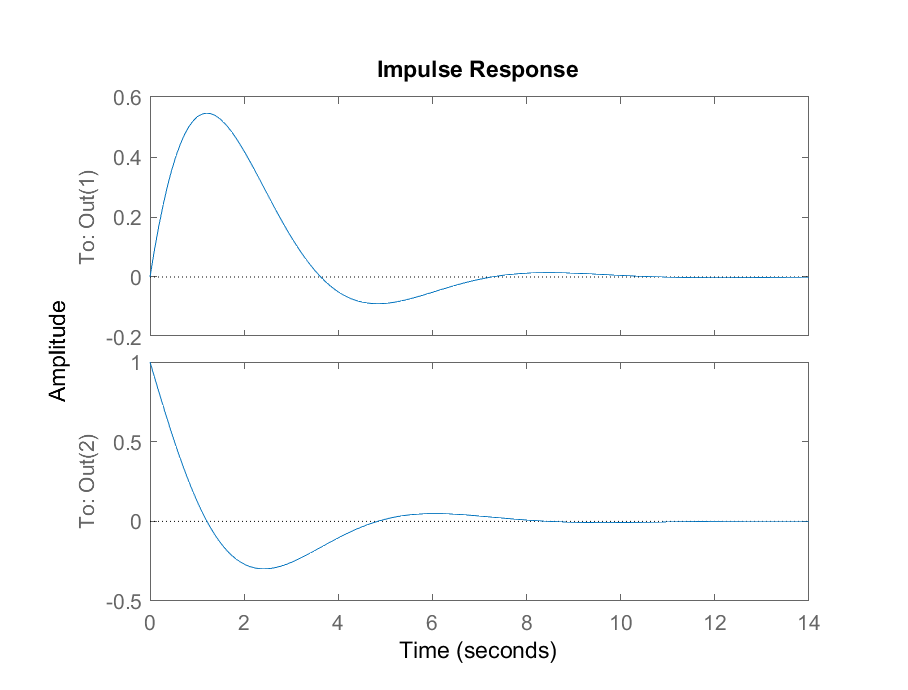
\includegraphics[width=0.7\textwidth]{impulse_response_msd.eps}
	\caption{Impulse response plot of the mass damper spring system.}
\end{figure}

Since we are considering the impulse responce of the system, we know that the input will be constant zero. Hence we will consider the system to be unforced for the time being. We will use the data to reconstruct the $A$ matrix of the system.

In the case of system identification we need that the matrix containing both $X_-$ and $U_-$ is full rank. Since our input data is constant zero we will not be able to identify the discrete time system matrices $A_d$ and $B_d$. However, due to our input being zero we are able to consider the system as if it had no input and hence we are able to identify the descrete time $A_d$ matrix. Note that for our state data to be compatible with the function from the toolbox we need to transpose is to be a wide matrix instead of a tall one.

\begin{lstlisting}
x = x';
[bool, A_d] = isInformIdentification(x)
\end{lstlisting}

Which will return that the data is indeed informative for system identification and gives us the following discrete time $A_d$ matrix.

\begin{equation*}
	A_d = \begin{bmatrix}
		 0.9959 &   0.0879 \\
		-0.0879 &   0.9080
	\end{bmatrix}
\end{equation*}

Now we need to verify that the continuous time counterpart of this descrete time $A_d$ matrix is indeed the same as our original system. For this we will use the function \mon{sysc = d2c(sysd)} provided by matlab to transform a discrete time system to a continuous time system. Note that we need to define a time step for our discrete time system, we can retreive the time step from the \mon{t} matrix returned by the impulse responce function.

\begin{lstlisting}
sys_d = ss(A_d, [], [], [], t(2));
A_c = d2c(sys_d).A
\end{lstlisting}

This will return the following continuous time $A_c$ matrix.

\begin{equation*}
	A_c = \begin{bmatrix}
		-0.0000 &   1.0000\\
		-1.0000 &  -1.0000
	\end{bmatrix}
\end{equation*}

As we can see our computed $A_c$ matrix is almost the same as the true $A$ matrix. The larges difference as computed by matlab between entries of the matrices is $0.3e-14$ which makes them the same up to machine precision.

\subsection{Step response}
We will now be considering the step responce of the system. We will pick our input to be constant $1$. Using this we will repeat the previous steps to see if we are able to accuratly recover both the $A$ and $B$ system matrices. We will generate the data using the built in Matlab function \mon{[y, t, x] = step(sys)}. 

\begin{lstlisting}
[~, t, x] = step(sys_c);
\end{lstlisting}

\begin{figure}[H]
	\centering
	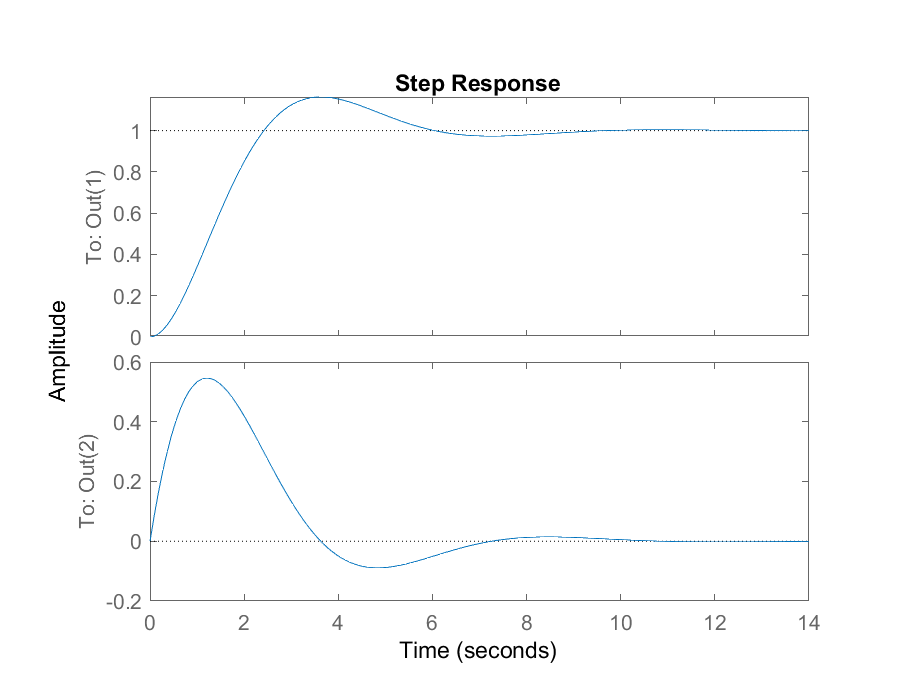
\includegraphics[width=0.7\textwidth]{step_response_msd.eps}
	\caption{Step response plot of the mass damper spring system.}
\end{figure}

Since our input data is non zero it might be the case that the matrix containing both $X_-$ and $U_-$ is full rank. Before we check if the data is informative for system identification we will prepare the data to be used for the toolbox.

\begin{lstlisting}
x = x';
U = ones(1,size(x,2) - 1);
[bool, A_d, B_d] = isInformIdentification(x, U)
\end{lstlisting}

From this we can indeed see that the data is informative for system identification and that the discrete time system matrices are given as:

\begin{align*}
	A_d &= \begin{bmatrix} 0.9959 & 0.0879 \\ -0.0879 & 0.9080 \end{bmatrix} &
	B_d &= \begin{bmatrix} 0.0041 \\ 0.0879 \end{bmatrix} 
\end{align*}

We will once again convert these to a continuous time system using \mon{sysc = d2c(sysd)} with the time step as defined in the \mon{t} matrix returned by the step function.

\begin{lstlisting}
sys_d = ss(A_d, B_d, [], [], t(2));
A_c = d2c(sys_d).A
B_c = d2c(sys_d).B
\end{lstlisting}

Which will return the following continuous time system matrices.

\begin{align*}
A_d &= \begin{bmatrix} 0.0000 & 1.0000 \\ -1.0000 & -1.0000 \end{bmatrix} &
B_d &= \begin{bmatrix} 0.0000 \\ 1.0000 \end{bmatrix} 
\end{align*}

As we can see the computed continuous time system matrices are again the same as the true system up to machine presision.
\newpage
%\section{How to use the toolbox for linearising models}\newpage
%\section{Improving controller performance using H$_2$}\newpage


% ----------------------------- Discussion and conclusion
\section{Conclusion}
The aim of this project was to implement the methods discussed in the informativity framework from \cite{waarde2019data} and \cite{waarde2020noisy} for computation of system theoretic properties and controller directly from data into Matlab as well as providing documentation for each methods.

This is done by providing a look at how the methods were derived in the documentation as well as providing corresponding functions for each method. This was done for all the methods described in the previously mentioned papers. The documentation also provides examples for each of the methods as well as an example of how the functions can be used for system identification on continuous-time systems using the impulse and step response. 

All these methods are implemented and available at: \\
\url{http://github.com/JeroenLam/Matlab-Toolbox-for-Data-driven-Control}

% ----------------------------- Future work
\input{31FutureWork}
% ----------------------------- Limitations -------------------------

% ----------------------------- Acknowladgements --------------------
\section{Acknowledgements}
I would like to thank dr. Henk J. van Waarde for his time and help with coordinating the project.
% ----------------------------- References --------------------------
%\section{Reference section title}
\printbibliography[heading=bibintoc,title={References}]
\todo{Fix S in dynamic measurement feedback}
% ----------------------------- Apendix ----------------------------- 


\end{document}



